% !TEX TS-program = pdflatex
% !TEX encoding = UTF-8 Unicode


\documentclass[10pt]{article} 

\usepackage[utf8]{inputenc} 
\usepackage{mciteplus}
\usepackage{multicols}
\usepackage{geometry}
\usepackage{cite}
\usepackage{caption}
\usepackage{subcaption}
\geometry{a4paper}
\usepackage{listings}
\usepackage{graphicx} % support the \includegraphics command and options

% \usepackage[parfill]{parskip} % Activate to begin paragraphs with an empty line rather than an indent
\usepackage{booktabs} % for much better looking tables
\usepackage{array} % for better arrays (e.g. matrices) in maths
\usepackage{paralist} % very flexible & customisable lists (eg. enumerate/itemize, etc.)
\usepackage{verbatim} % adds environment for commenting out blocks of text & for better verbatim
\usepackage{subfig} % make it possible to include more than one captioned figure//table in a single float
\usepackage{amsmath}
% These packages are all incorporated in the memoir class to one degree or another...

%%% HEADERS & FOOTERS
\usepackage{fancyhdr} % This should be set AFTER setting up the page geometry
\pagestyle{plain} % options: empty , plain , fancy
\renewcommand{\headrulewidth}{0pt} % customise the layout...
\lhead{}\chead{}\rhead{}
\lfoot{}\cfoot{\thepage}\rfoot{}

%%% SECTION TITLE APPEARANCE
\usepackage{sectsty}
\allsectionsfont{\sffamily\mdseries\upshape} % (See the fntguide.pdf for font help)
% (This matches ConTeXt defaults)

%%% ToC (table of contents) APPEARANCE
\usepackage[nottoc,notlof,notlot]{tocbibind} % Put the bibliography in the ToC
\usepackage[titles,subfigure]{tocloft} % Alter the style of the Table of Contents
\renewcommand{\cftsecfont}{\rmfamily\mdseries\upshape}
\renewcommand{\cftsecpagefont}{\rmfamily\mdseries\upshape} % No bold!

%%% END Article customizations

%%% The "real" document content comes below...

\title{Title TBC}
\author{Louie Corpe \\Supervisors: Paul Dauncey, Chris Seez }
%\date{}
%\hoffset = 0pt
%\voffset = -50pt
%\oddsidemargin = 0pt
%\topmargin = 0pt
%\headheight = 0pt
%\headsep = 25pt
%\textheight = 750pt
%\textwidth = 455pt
%\marginparsep = 0pt
%\marginparwidth = 0pt
%\footskip = 30pt

\oddsidemargin=0pt           % No extra space wasted after first inch.
\evensidemargin=0pt          % Ditto (for two-sided output).
\topmargin=0pt               % Same for top of page.
\headheight=0pt              % Don't waste any space on unused headers.
\headsep=0pt
\textwidth=16cm              % Effectively controls the right margin.
\textheight=24cm

\begin{document}
\maketitle

\renewcommand{\abstractname}{Abstract}
\begin{abstract}
{
An overview of the study of the Higgs boson via its decay to two photons at CMS is presented. A brief introduction into the history of the Standard Model and the motivation for Higgs searches is given, as well as a detailed description of the CMS experiment at CERN. The analysis of the $H \rightarrow \gamma\gamma$ decay mode is described in some detail, with reference to recent work. A discussion on the outlook and future work to be done in this decay channel is also given.}
\end{abstract}



\tableofcontents

\newpage 
%\begin{multicols}{2}
\section{Introduction}

The $H \rightarrow \gamma \gamma$ analysis played an important role in the discovery of the Higgs boson in 2012 (CITE FIXME), and has recently published an analysis using all of the data from run I (known as the ``legacy analysis''). This analysis has demonstrated the sensitivity of this decay mode: an observation of a Higgs boson signal with over $5 \sigma$ certainty allowed a standalone discovery to be claimed CITE LEGACY (FIXME - will be published?). My Ph.D. will involve working within this group, and helping run further studies on the Higgs boson's properties. 

In run II, the LHC will ramp up the centre of mass energy of collisions $\sqrt{s}$ to 13TeV and eventually to 14TeV. This increase, coupled with a rise in the luminosity of the beam (FIXME check!) should usher in the era of precision Higgs physics. The tradeoff to pay, however, is that further strain will be put on the trigger, reconstruction and event processing frameworks, both during data acquisition and after. For example, the number of additional (uninteresting) interactions within a bunch crossing, known as pileup, will increase, thus causing problems for triggering, track reconstruction and energy resolution. In order to make the most of the opportunities offered by run II, much work needs to be done to ensure that the CMS collaboration is ready to deal with these challenges when the LHC switches back on in March 2015, less than a year from now.

One example of where such work is required is in the calibration of the electromagnetic calorimeter (ECAL) subdetector. Because the $H \rightarrow \gamma \gamma$ analysis deals with photons, intrinsically electromagnetic objects, its sensitivity relies heavily on the performance of the ECAL. In run I, the excellent sensitivity of the subdetector allowed the analysis to play a  leading role in the discovery of the Higgs boson and the subsequent analysis of its properties. Naturally, in order to make further and more precise measurements in run II, the ECAL's performance must be improved, or at least maintained, despite the challenges of the $\sqrt{s} = 13$TeV environment.

To cope with these changes, the CMS collaboration has taken various steps. One of the key changes affecting the ECAL is an update of the CMS software, which reconstructs particles from the raw data. A holistic ``particle flow'' method is being implemented, allowing information from various subdetectors to be used in a holistic way. Specifically, this affects the reconstruction of electrons and photons within the tracker and ECAL: the way in which energy deposits are clustered with the array of ECAL crystals is being changed to allow more complicated shapes. This new reconstruction method has the advantage of being able to mitigate the effects of pileup, but represents a fundament shift in the treatement of electromagnetic objects. Although in principle this innovation should lead energy resolutions at least as good as those enjoyed by the ECAL in run I, it needs to be throughly tested and validated to ensure good performance in run II. Helping to validate this new clustering method is an aspect of the service work which I have pledged to complete, and intitial results will be presented.

Another important task, this time within the $H \rightarrow \gamma \gamma$ group specifically, is to publish a final analysis of the sensitivity achieved by the group's efforts during run I. In this way, it will be possible to learn from the experience of run I, and benchmark any potential improvements in the group-specific software and analysis tools. I was involved in one aspect of this work, namely the measurement of the individual photon energy resolution afforded by the $H \rightarrow \gamma \gamma$ software, \texttt{h2gglobe}. 

 This report is designed to communicate the research I have undertaken during the first nine months of my Ph.D. I present here the historical context of particle physics leading up to the modern day, an outline of Higgs physics at the LHC, and overview of the CMS detector as well as detailed account of my work and findings.





\section{The SM and $H \rightarrow \gamma \gamma$}

\subsection{The Standard Model}


The standard model (SM) of particle physics came into being in the mid-1970's, when the discovery of the $J / \psi$ particle~\cite{RichterPsi,TingJ} and results from deep inelastic scattering experiments at SLAC confirmed the predictions of quark models. The SM has been an immensely successful theory, accurately describing many processes in high energy physics. Among other features, the model placed all fundamental forces apart from gravity into one framework, and united the electromagnetic and weak forces into the electroweak force~\cite{GIM,Salam,Weinberg}. In order to do this, a mechanism was required to permit the $W^{\pm}$ and $Z$ vector bosons to have mass while allowing the photon to remain massless. Crucially, this process was required to preserve gauge invariance. Such a theory was independently proposed by several theorists~\cite{BroutEnglert,Higgs1,Higgs2,Kibble1,Higgs3,Kibble2}, and is commonly referred to as the Higgs mechanism. In 1964, Higgs postulated that one outcome of this mechanism was that it should yield an observable particle, the Higgs boson~\cite{Higgs2}. Over the decades, the particles postulated by the SM were discovered: the $\tau$ lepton in 1975~\cite{tauDisc}, the $b$ quark in 1977~\cite{bquarkDisc}, the gluon in 1979~\cite{Gluon1,Gluon2,Gluon3}, the $Z$ and $W^{\pm}$ bosons in 1983~\cite{ZDisc,WDisc}, the top quark in 1995~\cite{tquarkDisc1,tquarkDisc2} and the $\nu_{\tau}$ in 2000~\cite{TauNuDisc}. Each new discovery cemented the SM as one of the most successful theories of modern times. By the turn of the millennium, all but one particle postulated by the SM had been observed: the Higgs boson, which had proved elusive despite decades of searches. The Higgs search prompted the construction of the Large Hadron Collider (LHC) at CERN, and two multi-purpose detectors, ATLAS and CMS, were designed with the Higgs observation as one of their main physics goals. In 2012, the two experiments jointly announced the observation of a Higgs-like particle of mass $\sim$125 GeV, ending a 50-year lull between postulation and discovery~\cite{CMSHDisc,ATLASHDisc}.

Although the SM has been very successful as a theory, it falls short of being a “theory of everything", and is clearly incomplete. For instance, it does not accommodate mass terms for neutrinos, which are required to explain the origin of neutrino oscillations observed in many experiments~\cite{SuperK,SNO,DayaBay}. Furthermore, it does not contain a viable candidate for dark matter, which is needed to explain the mass deficit of the universe~\cite{DM}. Other issues such as the hierarchy problem~\cite{Hierarchy} and the origin of matter-antimatter asymmetry in our universe~\cite{Asymmetry} also persist. Clearly, the SM is incomplete or approximate, and many efforts in modern high energy physics are being made to discover “Beyond the Standard Model" (BSM) physics. Supersymmetry proposes one such extension to the SM, but many other models exist, and the search for new physics will be one of the primary objectives of experimentalists during run II of the LHC in 2015.

Even in the Higgs sector, more work remains to be done. Precision measurements of the properties of this particle are needed: does it behave like the SM predicts? Is there only one such particle? Detailed studies are required to ascertain couplings, the differential cross section, width and other attributes of this Higgs particle. Deviations from the expected values of such properties could provide valuable insight into the nature or indeed existence of BSM physics.

\subsection{$H \rightarrow \gamma \gamma$}
According to SM, the Higgs boson's coupling with particles is proportional to their mass. As such, its production modes in the environment of the LHC are dominated by interactions involving the heavier particles of the SM. Typically, the Higgs boson is produced by one of the following mechanisms, as illustrated in figure 2: a) gluon-gluon fusion, via a loop of top quarks, b) vector boson fusion (so-called “VBF"), with associated quark production, c) associated vector boson production (also known as “Higgsstrahlung") and d) top quark fusion with associated top quark production.
\begin{figure}[h!]


  \includegraphics[width=0.9\textwidth]{"test"}
  \caption{Higgs production mechanisms at the LHC.}
\end{figure}

By the same token, the SM Higgs boson decays to pairs of particles with branching ratios proportional to the square of their mass. The production of a pair of $t$ quarks is not kinematically allowed because their mass is high, so the most likely decay modes are $H \rightarrow ZZ \text{, } W^{\pm}W^{\mp}$, $ b\bar{b}$ and $ \tau^+ \tau^-$. In addition, a small fraction of decays of the Higgs boson ($<1\%$) can occur via a loop diagram to a pair of high-energy photons. The branching fractions and cross sections of these production and decay modes are available in the Handbook of LHC Higgs Cross Sections~\cite{H_XS1,H_XS2}.


\begin{figure}[h!]

  \centering
%\begin{subfigure}[b]{0.52\textwidth}  
%\includegraphics[width=\textwidth]{"Higgs_XS"} 
%\caption{Higgs production cross sections} 
%\end{subfigure}
%\begin{subfigure}[b]{0.4\textwidth}  
  %\includegraphics[width=\textwidth]{"Higgs_BR"}  
%\caption{Higgs decay branching ratios}
%\end{subfigure}
\includegraphics[width=\textwidth]{"SignalStrength"}
\caption{The signal strengths of the Higgs boson observation by decay mode and in combination at ATLAS (left) and CMS (right). The results are consistent with the observation of a particle of $m_H \sim 125$ GeV~\cite{H_XS3}.}
\end{figure}

The Higgs boson was discovered in 2012 using data from runs at $\sqrt{s}=7$ and $8$ TeV, and was found to have a mass $m_H \sim 125$ GeV. The signal strengths of the various decay modes at the CMS and ATLAS experiments can be seen in figure 3. Despite fewer than $1\%$ of Higgs boson decays occurring via $H \rightarrow \gamma \gamma$, this channel played a crucial role in the discovery, and remains one of the two most sensitive methods of studying the Higgs boson. This is in part thanks to the excellent performance of the CMS ECAL.




\section{The CMS detector}

\subsection{Overview}
The LHC is a synchrotron that was built in the tunnel which previously contained the Large Electron Positron (LEP) collider at CERN, near Geneva. It has a circumference of 27km and was designed to collide beams of protons (or lead ions) head on. In its latest run, it achieved a centre of mass energy of $\sqrt{s}=8$ TeV. The LHC shut down for a planned upgrade period in 2012, and is due to restart collisions in March 2015. At this stage, it should be able to deliver a centre of mass energy close to its design value of $\sqrt{s}=14$ TeV. 
As mentioned previously, the LHC is equipped with two multi-purpose detectors, CMS and ATLAS, which simultaneously discovered the Higgs boson using the data from run I. This report will focus on the CMS detector. The overall layout can be seen in the figure 1 below~\cite{CMSTDR}.
\begin{figure}[h]

  \centering
  \includegraphics[width=0.8\textwidth]{"CMSExploded"}
  \caption{The CMS detector perspective view.}
\end{figure}
CMS is a layered detector over 21m long and 14m in diameter, weighing over 12,500 tons. It consists of a superconducting solenoid magnet 13m long and 5.9m in diameter, generating a 3.8T magnetic field. On the outside of this, 4 layers of iron act as a return yoke, and house muon detector chambers (drift tubes in the barrel region and cathode strip chambers in the end cap region). The high magnetic field allows for good energy resolution in the compact space of the detector. The calorimeters and inner tracker are housed within the solenoid. 

\subsection{The tracker and the Electromagnetic Calorimeter}

The tracker and the electromagnetic calorimeter are the two subdetectors which the $H \rightarrow \gamma \gamma$ uses most (and indeed, almost exclusively). This report will therefore deal with them in a more detailed manner than it will for the other subdetectors.
The inner tracker consists of 4 layers of silicon pixel detectors close to the interaction region, surrounded by 10 layers of silicon micro-strip detectors. (INSERT MORE TRACKER INFO) These allow reconstruction of tracks and secondary vertices in the high track multiplicity environment of the LHC. The electromagnetic calorimeter (ECAL) is made up of an array of 61,200 lead PbWO$_4$ (lead tungstate) crystals in the barrel section and 14,648 crystals in the end caps~\cite{CMSTDR}. This is a central feature of the CMS detector as it allows for excellent energy resolution of incoming photons. The resolution of the ECAL is modelled with the equation \begin{equation} \left( \frac{\sigma}{E}\right) ^2= \left( \frac{S}{\sqrt{E}} \right)^2 + \left( \frac{N}{E} \right)^2 + C^2\end{equation} where $S$ represents the stochastic term, $N$ represents the noise terms and $C$ represents a constant term~\cite{CMSDesign}. The design values of these parameters are approximately $S=2.8\%$ GeV$^\frac{1}{2}$, $ N= 0.12$ GeV and $C=0.3 \%$. The performance of the ECAL matched these design values during the 2012 run~\cite{ECAL2012}. INSERT FIGURE of ecal performance?

\subsection{Other subdetectors}

The ECAL is then surrounded by a sampling hadronic calorimeter composed of brass/scintillator in the body and iron/quartz-fibre in the forward regions. The muon chambers INSERT INFORMATION ipseum loren Lorem ipsum dolor sit amet, consectetur adipiscing elit. Sed pharetra dapibus lorem sed mattis. Class aptent taciti sociosqu ad litora torquent per conubia nostra, per inceptos himenaeos. Etiam sollicitudin nisi in convallis interdum. Vivamus nec libero at nunc molestie elementum a et arcu. Curabitur facilisis felis eget condimentum mattis. Fusce tellus erat, porttitor aliquet porta at, rhoncus in justo. Aenean pretium nulla vel mi molestie imperdiet. Praesent aliquet velit nec ligula congue, eu lacinia orci ultrices. Mauris commodo cursus massa, ut cursus tortor consectetur eu. Suspendisse eu dictum odio. Morbi tincidunt ultrices erat in ultrices. 



\section{The $H \rightarrow \gamma \gamma$ analysis}

\subsection{Overview of the legacy analysis}

The $H \rightarrow \gamma \gamma$ analysis relies on the fact that there is a small but non-negligible branching fraction of Higgs bosons which decay to two highly energetic photons via loops of particles, generally virtual top quarks or $W^{\pm}$ vector bosons. Although around the mass $m_H \sim 125$ GeV there is a large irreducible QCD background, the excellent diphoton energy resolution ($\sim 1 \%$) of the CMS ECAL allows the reconstruction of a narrow peak above the background. The resolution available via this decay channel meant that it was identified early on as “one of the most promising channels in the search for a SM Higgs boson in the low mass range"~\cite{Seez}. The following description is based on the analysis of the $\sqrt{s}=7$ and $8$ TeV data samples~cite{HDisc}.

%Once candidate photon pairs are isolated, they are classed into mutually exclusive categories with different signal to background ratios. This allows the overall sensitivity of the analysis to be improved. These categories are distinguished by the properties of the reconstructed photons, and whether two jets were also recorded, corresponding to the VBF Higgs production mode. 
The analysis depends heavily on boosted decision trees (BDTs) to identify and classify events. A BDT is an algorithm which categorises items based on multiple input variables~\cite{BDT}. Different weights are applied depending on whether an item passes or fails cuts based on these input variables. The weights are summed at the end and the final value is used to determine which category the item falls in. The algorithm is trained (i.e. the aforementioned weights and cut thresholds are determined) with simulations or data with similar properties. %A day-to-day example of such an algorithm would be an email spam filter, where the items are to be classified as genuine or spam. The input variables would be, for example, frequency of exclamation marks or dollar signs, quality of spelling, use of the recipient's name. The output might be a value from 0 to 1 representing the probability that the email is spam, and above a certain value, the email would be directed to the relevant folder.

The first step in the analysis is to identify candidate diphoton events. There is a loose trigger, identifying any pair of photons in an event based on ECAL isolation, shower shape and energy. A more stringent selection takes place later to choose only diphoton events likely to have originated from a Higgs decay.
 
The next step is to locate the photon production vertex. This is an important step because an accurate determination of the origin of the photon tracks can be combined with the measured ECAL energies and spatial location of the photon showers to accurately reconstruct the Higgs 4-momentum, and thus its invariant mass. A simple analysis of conservation of 4-momentum in the laboratory frame yields the required formula:
\begin{equation} m_H=m_{\gamma\gamma}=\sqrt{2E_1 E_2 (1-\cos{\alpha})} \end{equation} where $m_{\gamma\gamma} $ is the invariant mass of the diphoton system, $E_{1,2}$ are the energies of the reconstructed photons and $\alpha$ is the opening angle between the two photons.
It is clear that since the ECAL resolution is excellent, $E_{1,2}$ are well known. The only other contribution to the mass resolution comes from the opening angle $\alpha$. In order to accurately measure this angle, the photon creation vertex must be identified to within 10 mm of its true position. If this is the case, the error contribution from $\alpha$ is negligeable.

Vertex identification can be achieved by matching the kinematic properties of the tracks coming from these vertices with the diphoton system's transverse momentum. Another option is to use information from the tracker if the photon converted into at $e^+ e^-$ pair: in this case the track directions can be combined with the impact position in the ECAL to extrapolate back to the photon production vertex. A BDT trained on simulated data is used to identify the vertex, using quantities such as those mentioned above as input variables. The vertex identification efficiency is measured to be of the order of 80$\%$, and the associated systematic uncertainty is well understood. 

Since the photon pairs expected from Higgs decay should be highly energetic, offline cuts are applied to select candidate diphoton events likely to have originated from a Higgs boson decay. These cuts are defined as $E_T > m_{\gamma \gamma}/3$ for one candidate photon and $E_T > m_{\gamma \gamma}/4$ for the other~\cite{HSearch}, where $E_T$ is the transverse energy of the photon and $m_{\gamma\gamma}$ is the invariant mass of the diphoton system. It is possible that a photon may have pair converted ($\gamma \rightarrow e^+ e^-$) before reaching the ECAL. Such occurrences are identified using the variable $R_9$, defined as the sum of the energy of the $3 \times 3$ array of lead tungstate crystals centred around the most energetic crystal in the supercluster, divided by the total energy of said supercluster. A value of $R_9$ smaller than $0.94$ is indicative of a photon having undergone pair conversion. $R_9$ is used as an input variable in a BDT which classifies events based on their sensitivity, as described below. A further BDT is also used to remove “non-prompt" photons (i.e. photons not created at the primary vertex) and other particles misidentified as photons, such as pions.

The events are then segmented into categories based on the expected signal to background ratio and diphoton invariant mass resolution. Studying these separately increases the overall sensitivity of the analysis. An additional categorisation where candidate events also pass a dijet trigger corresponds to VBF Higgs production (See figure 2.b: the quarks are scattered at a sufficiently large opening angle for them to undergo hadronisation and form jets rather than be lost down the beam-pipe). This mode is analysed separately because its signal to background ratio is over an order to magnitude better than for the other categories~\cite{HSearch}. The categorisation is achieved using another BDT, where the input variables are chosen to be dimensionless to avoid any bias in the mass distribution. For example, the transverse momenta of the photons are used amongst other input variables, but they are scaled by the calculated diphoton invariant mass to yield a dimensionless criterion.

The background model is obtained using a data-driven technique rather than a MC prediction, as this avoids any systematic uncertainties based on mis-modelling. For each of the categories, the diphoton mass distribution outside of the region of interest is fitted. The function used to fit the data is chosen based on minimisation of the bias introduced in each case. Candidate functions involve exponentials, power laws, polynomials and Laurent series. The bias is found to be negligible when Bernsteins of order 3 to 5 (depending on the category) are used.

Finally, the observed invariant mass distribution is compared to that predicted by the background fit. An observed excess of events around $\sim125.0$ GeV with a local significance of $4.1 \sigma$ in the $\gamma \gamma$ decay channel signalled the existence of the Higgs boson in 2012. Combined with measurements from other decay modes, CMS anounced a measuremement of $m_H=125.3 \pm 0.4 \text{(stat.)} \pm 0.5 \text{(syst.)}$ GeV with a local observed significance of $5.0 \sigma$~\cite{HDisc}.


\subsection{Photon resolution studies}

\subsubsection{Motivation}

An important task after the publication of the legacy analysis is to learn lessons from the perofmrance of the previous run. This allows better preparation for run II. As such, a paper is being prepared to mark the performance of the $H \rightarrow \gamma\gamma$ software during the later part of the first run. One aspect of this was to run a study to look at the resolution of photon energies as reconstructed using the globe software package. I was tasked with repapring this plot.

The study consisted of looking at the reconstruction of Higgs boson decay photons in simulated collision at 8TeV, assuming $m_H = 125GeV$. The resulting plot was intended to give the effective energy resolution $\sigma_{\text{eff}}/E$ for individual photons, given in small $|\eta|$ bins.
Monte Carlo samples for the $8TeV$ LHC condidtions were used in this study. More precisely, a sample of simulated $H \rightarrow \gamma \gamma$ events corresponding to each Higgs production mode (Vector Boson Fusion , Glugon-Gluon Fusion, Associated Vector Boson Production and Associated Top Quark Production), weighted by cross section, were used as the dataset for the study.
Since the intention is to provide an account of the sensitivity of the $H \rightarrow \gamma\gamma$ analysis, the MC samples were passed through the globe MVA framework, and therefore were processed as they would have been in the legacy analysis, with full smearing and correcttions.



\subsubsection{Method and Result}

In order to produce the required plots, the globe MVA framework code was modified so as to produce an additional root tree, containing only the information needed for this study. The writing of this additional tree took place after all the actual analysis within the framework was complete. In order to measure the effective energy resolution of the photons, it was necessary to compare the ``true'' energy of the photons $E_{true}$(as generated in the simulation) with the ``reco'' energy of the photons $E_{reco}$ (as provided after reconstruction and application of corrections in the the globe framework). To make this comparison in a meaningful way, the generated photons and the reconstructed needed to be matched correctly. This was done using an unambiguous geometrical method: for each generated photon in an event, the value of $\Delta R = \sqrt{\Delta \eta^2 + \Delta \phi^2}$ (where $\Delta $ refers to the difference between generated and reconstructed values) was calculated for the two reconstructed photons. The reconstructed photon minimising the value of $\Delta R$ was chosen as the match for that generated photon. (DELTA R and DELTA ETA PLOTS??)

For each event, each individual photon was categorised first by $R_{9} <0.94$ or $R_{9} \geq 0.94$, then  by its value of $|\eta|$. The width of the $|\eta|$ categories was 0.1, apart from the region near the transition between the ECAL barrel and ECAL encap, where the data are excluded (resulting in two slightly larger categories on either side, namely $ 1.3 \leq |\eta| < 1.4442 $ and $1.566 \leq |\eta| < 1.7$), thus 23 categories. Taking into account the two $R_{9}$ options, this left 46 photon categories. For each one, a histogram of the values of $E_{reco}/E_{true}$ was created. An algorithm is used to calcluate $\sigma_{\text{eff}}$ (defined as half the width of the smallest window containing 68.3\% of events in a distribution). This algorithm recursively scans potential windows in the histogram until the smallest mathcing the required condition is found. A different algorithm also calculates  the ``Full Width Half Maximum'' (FWHM), which is the width of the peak when measured at half of its maximum height. In this case , the algorithm fits each histogram to a combination of a Gaussian and a Crystal Ball function (AVAILABLE IN APPENDIX), then creates a very finely binned histogram of the best fit, and finds the bin with the largest number of events. Then it finds the first bin with half that number of events, and the last bin with half the number of events. For a true Gaussian distribution, $\sigma_{\text{eff}} = \sigma = \text{FWHM}/2\sqrt{2\ln2} \simeq \text{FWHM}/2.35$. In other cases, $\sigma_{\text{eff}} \geq \text{FWHM}/2.35$. Fig. 4 shows examples of these histograms. 

\begin{figure}[h!]

  \centering
\includegraphics[width=0.48\textwidth]{"Hist2_mva"}
\includegraphics[width=0.48\textwidth]{"Hist25_mva"}
\caption{Example $E_{reco}/E_{true} $ histograms for two $|\eta|$ and $R_{9}$ categories. The vertical axis indicates the number of events if each event were counted with the weight associated to a GGH event. Overlayed on each plot is the calculated value of  $\sigma_{\text{eff}}$ and $\text{FWHM}/2.35$. For a distribution with a Gaussian peak but non-Gaussian tails, we expect $\sigma_{\text{eff}} \geq \text{FWHM}/2.35$, which is what is observed.}
\end{figure}

The values of FWHM are not used in the rest of the study, however they provide a good sense check that the distributions make sense. On the other hand, $\sigma_{\text{eff}}$ is used as the input for the main result. The values of $\sigma_{\text{eff}}$ for the distributions of  $E_{reco}/E_{true}$ are equal to $\sigma_{\text{eff}}/E$ (FIXME why??), and are used as inputs to the effective energy resolution plot. Each of the 46 $|\eta|$ and $R_{9}$ catgeories provide a value, which is then plotted versus $|\eta|$ to give the main plot (Fig.5).

As epxected, the effective resolution is concistently worse for low $R_{9}$ categories than for their high $R_9$ equivalent. This is because low $R_9$ photons are likely to have undergone pair conversion, and the resulting electrons and positrons may have emitted energy via bremmstrahlung before hitting the ECAL. Furthermore, the categores where $|\eta|$ lies over a supermodule boundary (vertical dashed lines) have worse resolution than neighbouring categoreis. This is also expected, as the interfaces between teh supermodules are less hermetic than the body of teh supermodules, leading to energy lost between the gaps. Finally, the resolution in the endcaps (ie categoreis where $1.5\leq |\eta| <2.5$) is substantially worse than fhe resolution in the barrel. This is also expected (FIXME wy??).
In conclusion, this study set out to estimate the individual photon resolution in small $\|eta|$ bins in the CMS ECAL for simulated $H \rightarrow \gamma \gamma$ events at $m_H =125$GeV, after the full and final corrections applied with the globe framwork. The result is that for high $R_9$ photons in the barrel, the effective energy resolution is of the order of $/sim 1\%$ in the barrel and $\sim 2/4\%$ in the encaps. For low $R_9$ photons, the resolution is slightly worse.
\begin{figure}[h!]

  \centering
\includegraphics[width=0.9\textwidth]{"EffSigma_vs_eta_mva"}
\caption{$\sigma_{\text{eff}}/E$ plotted against $|\eta|$. Horizontal dotted lines shown as guides only. Vertical dashed lines show boundaries between supermodules. The grey band indicates the interfact between the ECAL barrel and encap regions, which we do not study. Horizontal error bars indicate width of $|\eta|$ bin, while vertical error bars (visible chiefly in the high $|\eta|$, low $R_{9}$ categories), indicates the estimated uncertainty on the measurement of the resolution. }

\end{figure}
\subsubsection{Estimation of the error}
The veritcal error bars in Fig. 5 provide an estimate of the uncertainty associated with the measurement of the resolution in each $|\eta|$ and $R_9$ category. The error for a given $|\eta|$ and $R_9$ category was assumed to be at least as large as the standard stastical error, given by $\text{Err}_{\text{stat}} = \sigma_{\text{eff}}/\sqrt{2N}$ (where $N$ is the number of photons in the category). However, additional uncertainty may have been added by the algorithm. To check this, the sample was divide into ten equivalent subsamples. For each subsample, the entire study was rerun, and the resulting ten values of $\sigma_{\text{eff}}/E$ were recorded for each of the 46 $|\eta|$ and $R_9$ categories. The RMS of these ten values was calculated in each case. If the error really were equal to $\text{Err}_{\text{stat}}$, we would expect that the subsample RMS error in each category would be $\sim \sqrt{10} \simeq 3.2$ times larger than the error for the full sample. However, when comparing the caluclated subsample RMS error to the minimum statsitical error for each category, the factor was on average 4.4 rather than 3.2, indicating that the true error is (very roughly) $~1.5$ times larger than $\text{Err}_{\text{stat}} $. As a result, the error added into Fig. 5 was $\text{Err}_{\text{stat}} \times 1.5$, thus providing a rough estimate of the uncertainty of the resolution. For most bins, the fact that $N$ is very large means that the veritcal error bars are completely invisible, however for low $R_9$, high $|\eta|$ categories, which have fewer photons, the error bars are no longer negligeable.

\subsubsection{Checks}

Several checks were performed during the course of the study in order to verify the consistency of the results. The main ones are summarised here. Firstly, the photon matchign mechanism was checked thoughly. The good performance of the matchign mechanism can be seen in Fig. 6.

\begin{figure}[h!]

  \centering
\includegraphics[width=0.9\textwidth]{"Delta"}
\caption{ The plot on the left (right) shows $\Delta \eta$ ($\Delta \phi$) for photons used in this study, where $\Delta X$ refers to the difference between $X_{\text{reco}}$ and $X_{\text{true}}$. The resulting distributions are very narrowly centered about 0, showing that the matchign algorithm is perfoming very well. In the rare cases where $\Delta \eta$ and $\Delta \phi$ are different from 0, this is due to poorly reconstruction of photons rather than mismatching.   }
\end{figure}
Secondly, the, the study was run using the CiC (REFER EARLIER FIXME) globe framework, rather than the MVA globe frmaewokr. Sicne the CiC framework was used as a crosscheck for the MVa frmaewokr in the actual lagacy anaylis, it provided and excellent opportuinjty to check consistency in this study. As can be seen in Fig. 7, the CiC version leads to slighly worse resolution in the endcaps, which is as expected since the MVA framework was designed to be more sensitive in this region.

\begin{figure}[h!]

  \centering
\includegraphics[width=0.4\textwidth]{"EffSigma_vs_eta_mva"}
\includegraphics[width=0.4\textwidth]{"EffSigma_vs_eta_cic"}
\caption{The plot on the right (left) shows the final result when the initial data are run through the globe CiC (MVA) framework. The results are almost indetical, with the biggest differences obsevrable in the low $R_9$, high $|\eta|$ categories. This is as expected, as the MVA analysis was designed to be more sensitive, especially in this region.}
\end{figure}

A Final check was run to check whether modifying the binning in of the $E_{\text{reco}}/E_{\text{true}}$ plots had an effect on the result of the $\sigma_{\text{eff}}$ algorithm. Various bin sizes were considered, however, the change in the resulting values of $\sigma_{\text{eff}}$ were less than negligeable (at most 1.7\% in the most extreme cases).








\section{ECAL calibration and service work}
\subsection{Overview of the task}

The overall collection of CMS Software is called CMSSW. \textit{``The overall collection of software, referred to as CMSSW, is built around Framework, an Event Data Model, and Services needed by the simulation, calibration and alignment, and reconstruction modules that process event data so that physicists can perform analysis.``}~\cite{CMSSW}

Effectively, CMSSW provides a way to process and select events from the raw data and allow physicists in the CMS collaboration to analyze the outcome and procude physics results. One way in which CMSSW does this is in the reconstruction of particles. Of particualr interest to the $H \rightarrow \gamma \gamma$ group is the way in which photons are reconstructed within the ECAL. The latest version of CMSSW is known as CMSSW\_7\_0\_X, where the X can represent a number of different sub-versions. A key distinction between this and the version used during run I (known as CMSSW\_5\_3\_X) is indeed the way in which photons are reconstructed. In the new version, a ``Particle Flow'' (PF) (FIXME explain??) approcach has been been implemented. Using the new PF clusters, CMSSW\_7\_0\_X applies the so-called ``moustache clustering'' method, so called because of teh shape of the energy distributions woth respect to the seed crystal (effectively,the new method uses more conplex shapes that simple boxes around crystals, as used in teh preivous ietration). (FIXME picture? more explnatation needed). In this method, all ECAL objects (electrons and photons) are reconstructed with the algorithm and udnergo particle identification as a different time. This method was implemented because it is able to take advamtage of the ECAL granularity to improve conatianment of electrons and photons while rejecting pileup. Advanatges of the method also include better low-$p_T$ electron resolution, particle-based isolation... 

However, although in principle the mew clustering method should provide many advnatgaes, it needs to be validated. Any significant loss in the energy resolution of ECAL objects could have a potentially disastrous effect on the $H \rightarrow \gamma \gamma$ anaylysis in particular, but in general CMS's capability to make important measurements in run II. My service work therefore is to work with the ECAL detector performance group (DPG) to help cehck the performance of CMSSW\_7\_0\_X against the perofmrance of CMMSSW\_5\_3\_X. 

\subsection{The ECALELF tool}

The \textbf{E}CAL \textbf{Cal}ibration with \textbf{El}ectron \textbf{F}ramework is a generic tool which uses $Z \rightarrow e^+ e^-$ events to monitor and calibrate the ECAL. ECALELF works within CMSSW to provide aligned and calibrated data upon which tests and studies can be run. In this sense, it is an ideal tool to test the new clustering method for electrons, and can be adatpted to validate teh reconstruction of photons also. The general workflow for calibration with ECALELF is to take $RECO$ data and MC  (ie, raw data which has been reconstricted using the native CMSSW version) for a given set of conditions , and apply a selection to retrieve only candidate $Z \rightarrow e^+ e^-$ events. A further selection is made via  BDT to reduce to pool of candidate events. Once this is complete a map between MC and data events based on finely segmented $\eta$ and $R_9$ categories. In general, the two electrons in a candidate event will not belong to the same category. In this case, it is difficult to know what correction factor needs to be applied to the enrgy of each electron in order to obtain the correct inbvariant mass distribution. Howeverm when both electrons in the candidate event belogn to the same $\eta$ and $R_9$ category, once can look at the MC invariant mass distribution in that category, compare it the invariant mass distribution of the candiate data events in that catgeory, and infer thet the correction to be applied to electrons (as a function of energy) in order to retireve the required distribution. In this way, $Z \rightarrow e^+ e^-$ events with both leptons in the same category allow teh calclulation of the requried correction (as a function of energy) to be applied to \textit{individual} electrons in that category. Once this has been done for all categopries, the events where the electrons/positrons belong to different categories can also be corrected (since each one will belong to a category where there requried correction for an individual electron is known). The result will be a set of corrections to apply in any $\eta$,$R_9$ scenario, thus providing the calibration. This ios known as the ``smearing method''.

Apart from atcual calibration, the ECALELF tool can be used to run general studies one Ecal performance using the output data from the setp before the application of the smearing meothod. Namely, one can  theoritcally comapre the ECALELF ntuples resulting from different CMMSSW releases, since the ntuples will be in the same format.


Although ECALELF provides an opportunity to test the performance of the new clustering method by comapring it to the previous release's ntuples, work needed to be done in order to make ECALELF work in the new CMSSW environment. Various variables had changed from one version to the other, it an update of teh software was needed. However, it oerder to run a proper conparison, a version of ECALELF which functioned within both 53X and 70X was needed. In other words, we needed to develop code which could activelyd etect which CMSSW version was beign used, and make the required subsitutions at compile time. I carried out this work and compleyted it in the first quarter of 2014.

\subsection{CMSSW\_7\_0\_X and CMSSW\_5\_3\_X electron matching}

As mentioned previously, the output of ECAELEf provides a good starting point to compare the performances of CMSSW\_7\_0\_X and CMSSW\_5\_3\_X in reconstructing ECAL objects. Although it deals with $Z\rightarrow e^+ e^-$ events, the calibration can also be applied to photons by reconstructins electrons asn photons, and using photons from the elctron showers. The advnmatge of using ECALELF ntuples is also that the output from both reconstructed datasets is in an identical fromat once passed through the machinery.

Ideally, both MC and Data from both CMSSW versions would be available, to run the ECALELF tool fully, and work out the best set of corrections to be applied in each case. A re-reconstruction of the full 2012 Run I dataset using the 70X framework was completed in april. However, at the present time, the MC for 70X is not yet available, so prelimianry studies are limited to comparing data in 53X and data in 70X. The objective will be to run a deeper validation once all the required samples become available.

In the meantime, since the data samples processed with 70X and 53X represente the same udnerlyong raw event samples, there is an opprotunity to compare some basic quantities electron-by-electron. The idea is to match electrons in both samples, and thereby to be able to distributions of the fratcioanl changes and differences between the qauntoities in eahc of the two frameworks. 

(FIXME INSERT TABLE WITH SAMPLE NAMES)

The first step, howeverm was to amend ECALELF to procude such a map. In teh ususal use case, ECALEF is designed to take as input one MC and one data sample. The tool therefore had to be modified to accept two data inputs. PArt of my work was to write the algorithm which would match the electrons in one sample with the elctrons in the other. The difficulty is that electrons within events might not be reconstructed in the same order, so for each entry in the first sample, all of the entries in the scond sample neeeded to be scanned for candidates. Given the large number of electrons in any of the run I samples, a consideration was to ensure that running such a program did not take an unreasonable amount of time. To speed up the process, the fact that runNumber and eventNumber of corresponding electrons in eahc sample should match was employed. Another trick was to store a list of all allowed candiate entries in a vector, and then to remove an already-matched entry in case of a match, so that the enxt ietration did not need to scan over events which had already been assigned. Originally, a simple entry-by-entry rejection of entries which did not have a matching eventNumber and runNumber was used, however this version of the programme took $>10$hv to process one of the subsamples. A modificationw as introcuued, which used a new user-defined class compirsing of \texttt{eventNumber} and \texttt{runNumber}  and  a \texttt{std::multimap} class (which replaced the \texttt{vector} in the previous version). The \texttt{std::multimap} class is useful because it allows elements to be mapped to a ``key''. The ``key'' can be used to access the elemts of the texttt{std::multimap}, and especially usefylly, if mutiple entries have the same ``key'', teh class can return a range which can be iterated over. In our case, the new class comprising of ordered \texttt{eventNumber} and \texttt{runNumber} pairs was used as the key for the  \texttt{std::multimap} of candidate entries, allowing the iteration over relevant entries only, rather than iteration over all entries with case-by-case rejection of entries with the worng \texttt{eventNumber} and \texttt{runNumber}. With this new method, the matching of one subsample took around $10$min, and found macthes for $\sim 80\%$ of electrons. (FIXME provide explanation as to why the other 20\% didn't get matched). Teh programme was also able to tell if the order of electrons within an entry was switched, and record this information for use later. The information is stored in a new \texttt{TTree} which stores, for every entry in one tree, whhat the corresponding entry in teh second tree is, and whetehr the order of electrons has been reversed. If no match is found, the entry in teh second \texttt{TTree} is recorded as $-1$.

\subsection{Initial validation work}

With the two data samples and the disctionary \texttt{TTree} linking them, it was possible to begin comparing quantities from one framework to another. Sme of teh basic qunaitites which I was asked to comapre for the two were: the reconstructed electron Energy, the electron $R_9$, the reconbstructed electron $\eta,\phi$ coordinates, the  $E/p$, the fraction of energy emitted in bremmstrahlung and the invariant mass of the $Z$ boson peak.

\subsubsection{Energy}
\begin{figure}[h!]
        \centering
        \begin{subfigure}[b]{0.4\textwidth}
                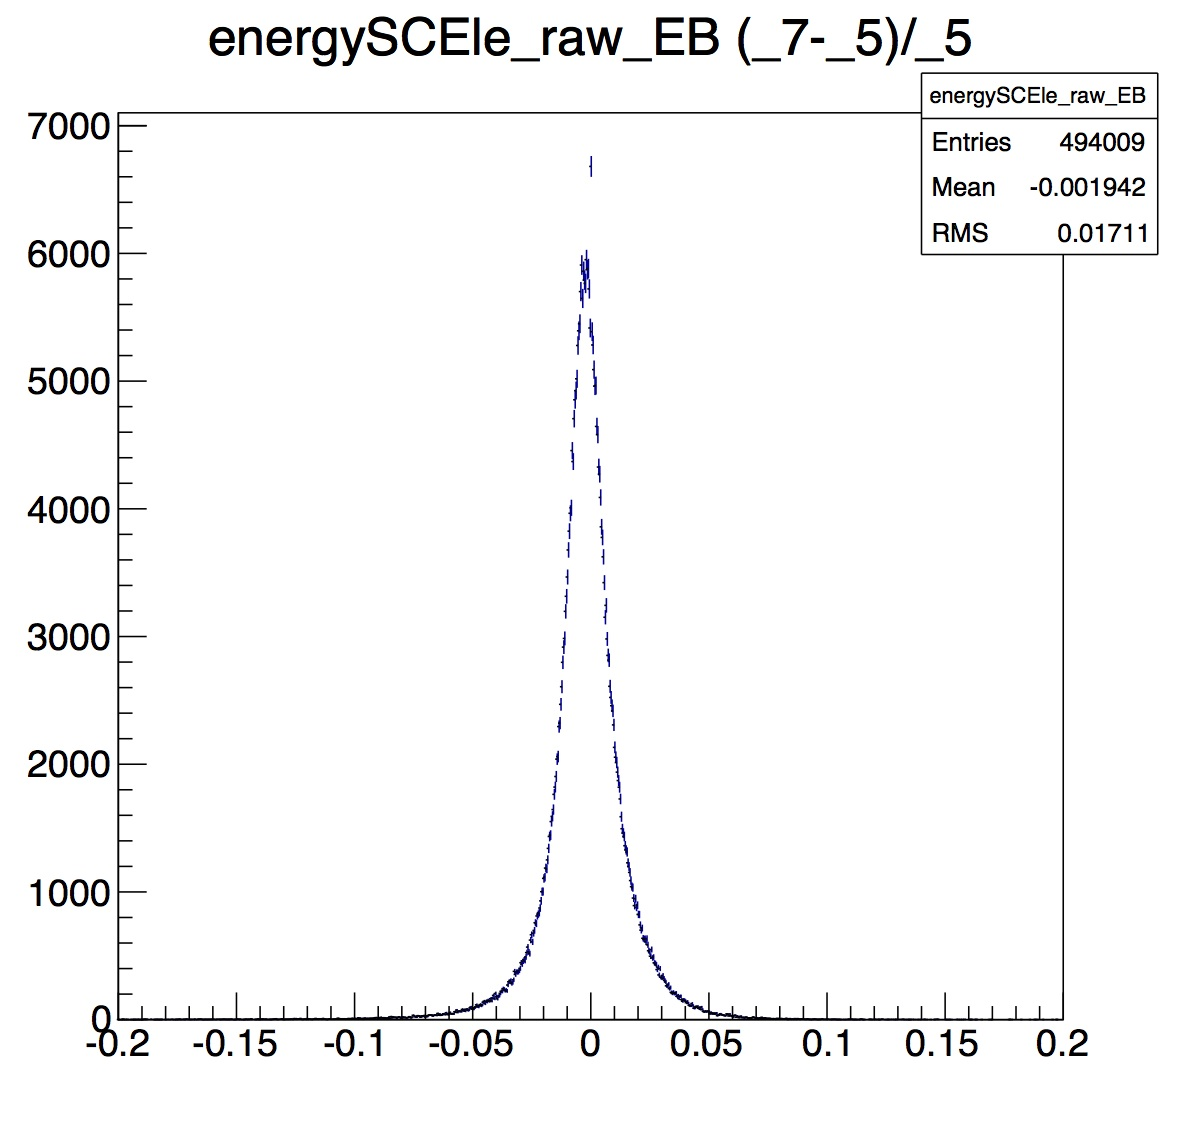
\includegraphics[width=\textwidth]{Plots/rawEnergySC_EB}
                \caption{A gull}
                \label{fig:gull}
        \end{subfigure}%
        ~ %add desired spacing between images, e. g. ~, \quad, \qquad, \hfill etc.
          %(or a blank line to force the subfigure onto a new line)
        \begin{subfigure}[b]{0.4\textwidth}
                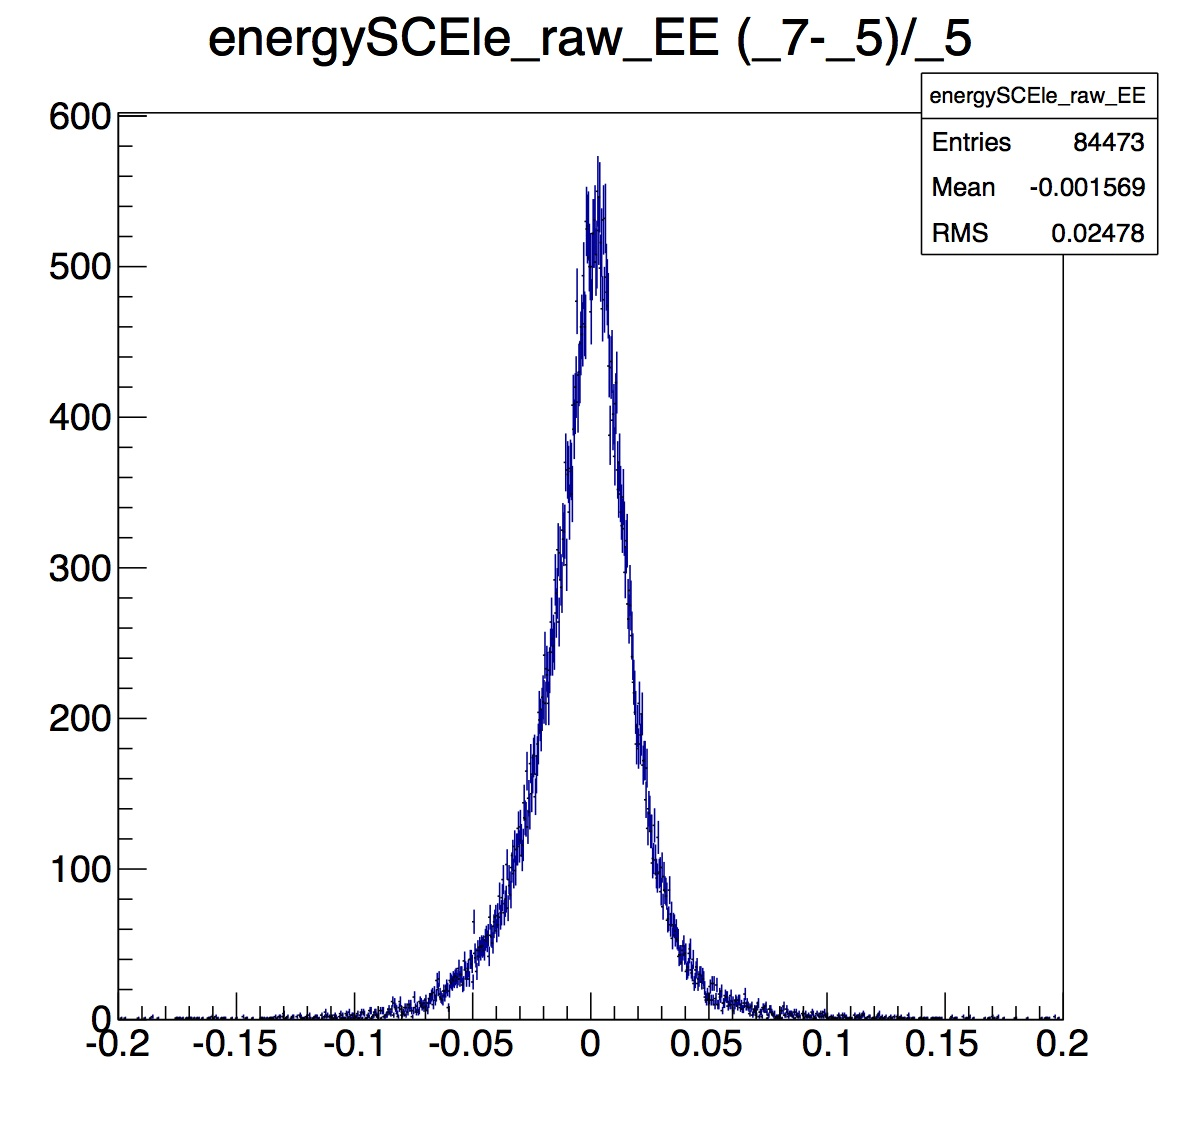
\includegraphics[width=\textwidth]{Plots/rawEnergySC_EE}
                \caption{A tiger}
                \label{fig:tiger}
        \end{subfigure}
        ~ %add desired spacing between images, e. g. ~, \quad, \qquad, \hfill etc.
          %(or a blank line to force the subfigure onto a new line)
        \begin{subfigure}[b]{0.4\textwidth}
                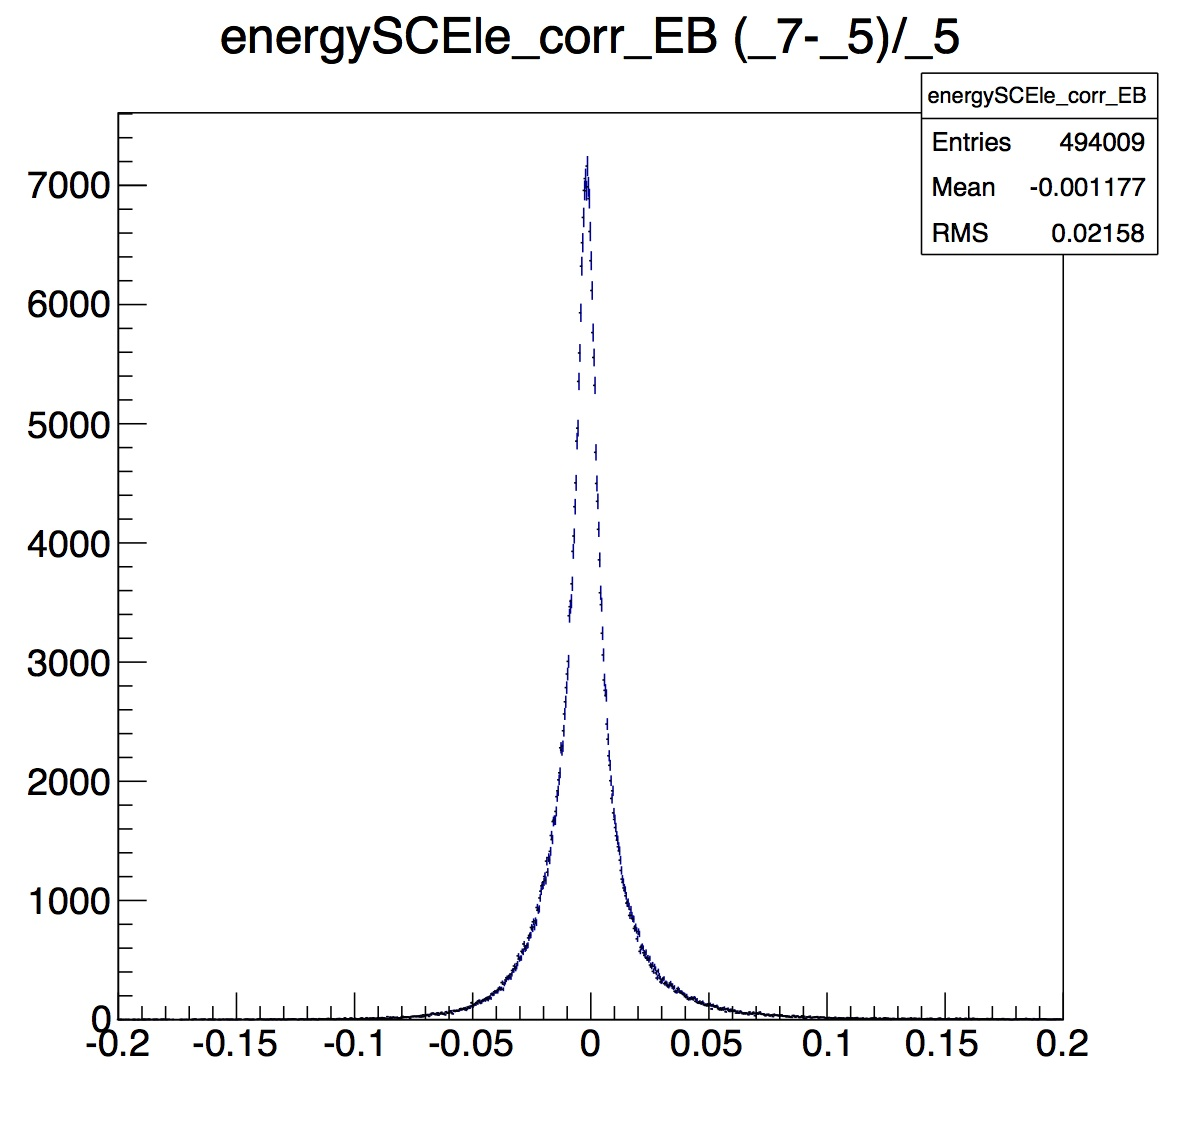
\includegraphics[width=\textwidth]{Plots/corrEnergySC_EB}
                \caption{A mouse}
                \label{fig:mouse}
        \end{subfigure}
         \begin{subfigure}[b]{0.4\textwidth}
                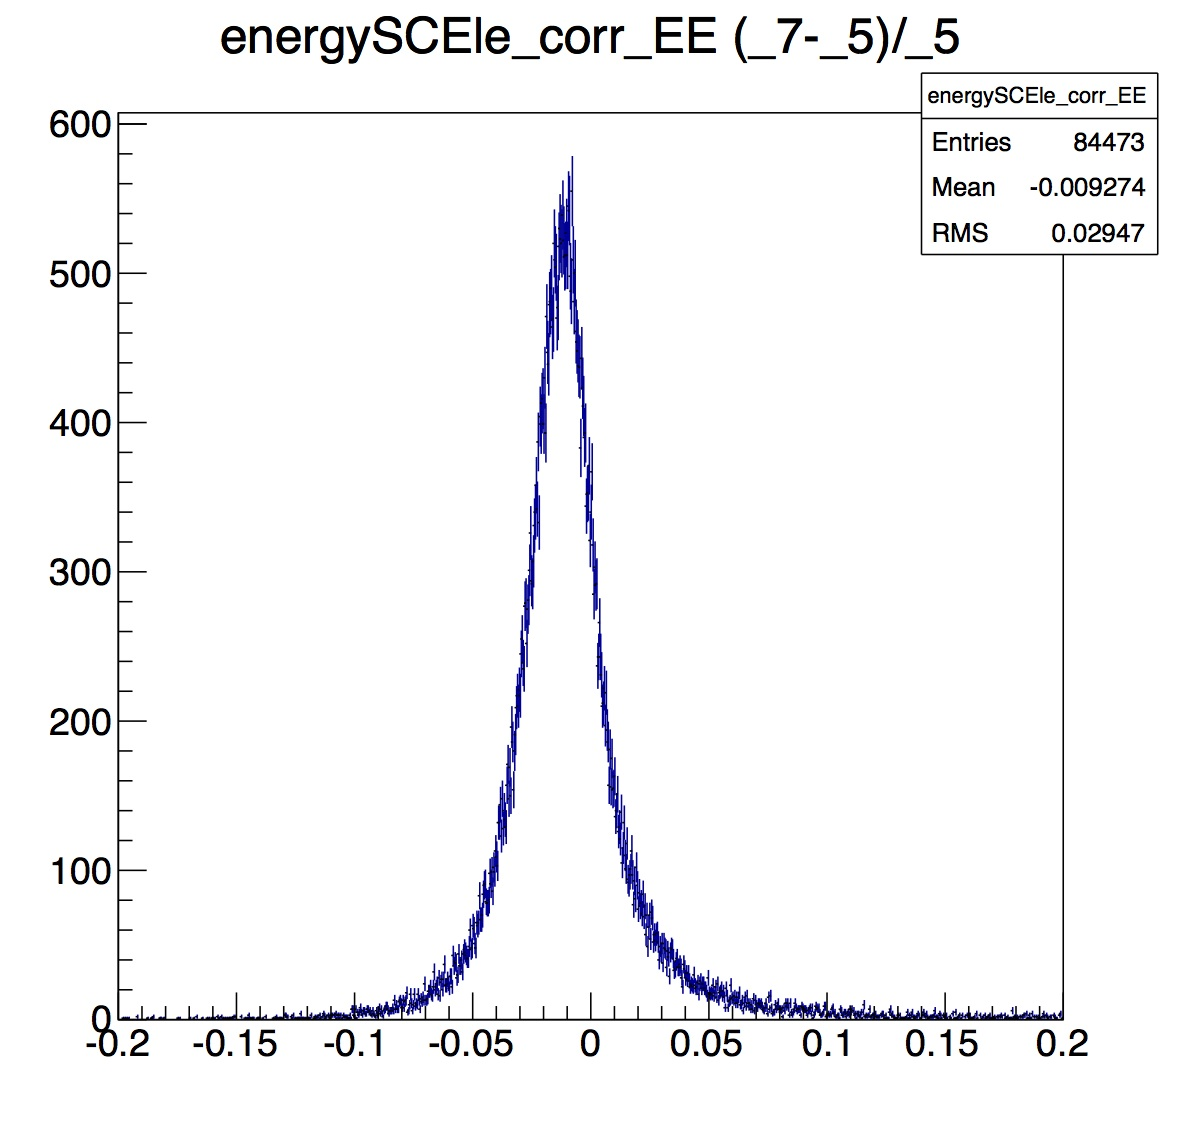
\includegraphics[width=\textwidth]{Plots/corrEnergySC_EE}
                \caption{A mouse}
                \label{fig:mouse}
        \end{subfigure}
        \caption{Pictures of animals}\label{fig:animals}
\end{figure}

The reconstruction of the energy of ECAL objects is clearly of paramount interest in this study. Fig. 8 shows the fractional energy difference $(E_{70X}-E_{53X})/E_{53X}$ for two different estimations of energy: the raw energy (Fig. 8.a) and 8.b)), which is simply the sum of the enrgies in the crystals forming the cluster, and the corrected energy (Fig. 8.c) and 8.d)), which is the ``best estimate'' using the most sophisticated regression available for each model. In the latter case, the corrected energy for 53X is the ``best'' option available, while the corrected energy for 70X is simply an initial attempt at correction, which is likely to imrpove greatly once the the sample is calibrated using the MC. The figures are split between ECAL endcaps (EE) and barell (EB). The figures indicate that the average chnage between the corrected energies in the EB is of the order of $\sim 0.12\%$, and in the EE of the order of $\sim0.3\%$. However, this is only a preliminary result and needs to be further examined. For instance, it needs to be understood whether teh ``corrected' energies'' used actually provide a fair comaprison, as this is far from being the best option for 70X in particular.

\subsubsection{$E/p$}
\begin{figure}[h!]
        \centering
        \begin{subfigure}[b]{0.4\textwidth}
                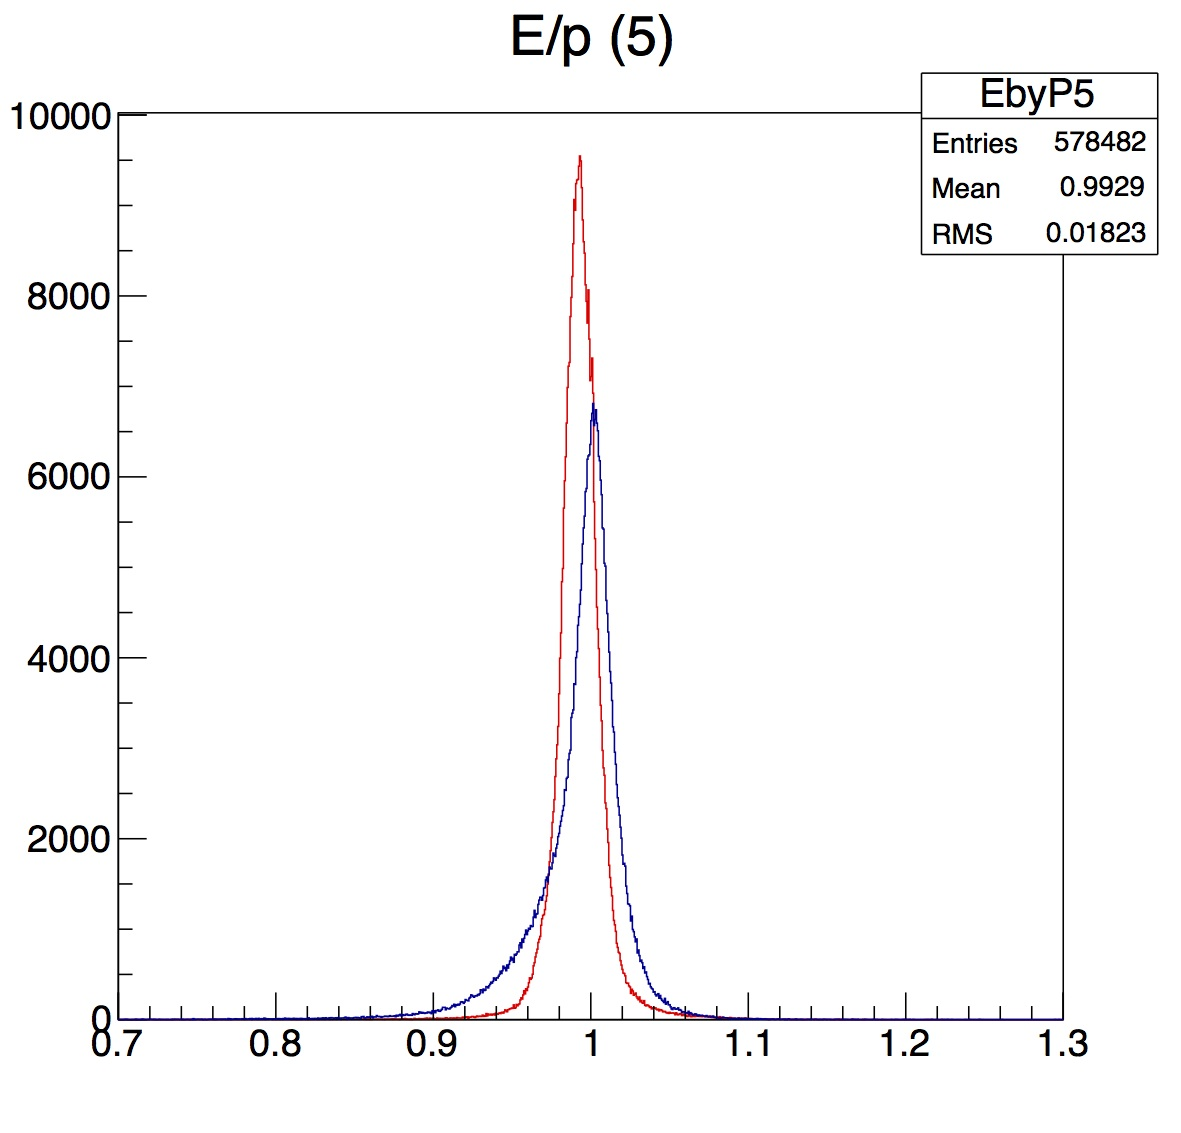
\includegraphics[width=\textwidth]{Plots/EbyPdist}
                \caption{A gull}
                \label{fig:gull}
        \end{subfigure}%
        ~ %add desired spacing between images, e. g. ~, \quad, \qquad, \hfill etc.
          %(or a blank line to force the subfigure onto a new line)
        \begin{subfigure}[b]{0.4\textwidth}
                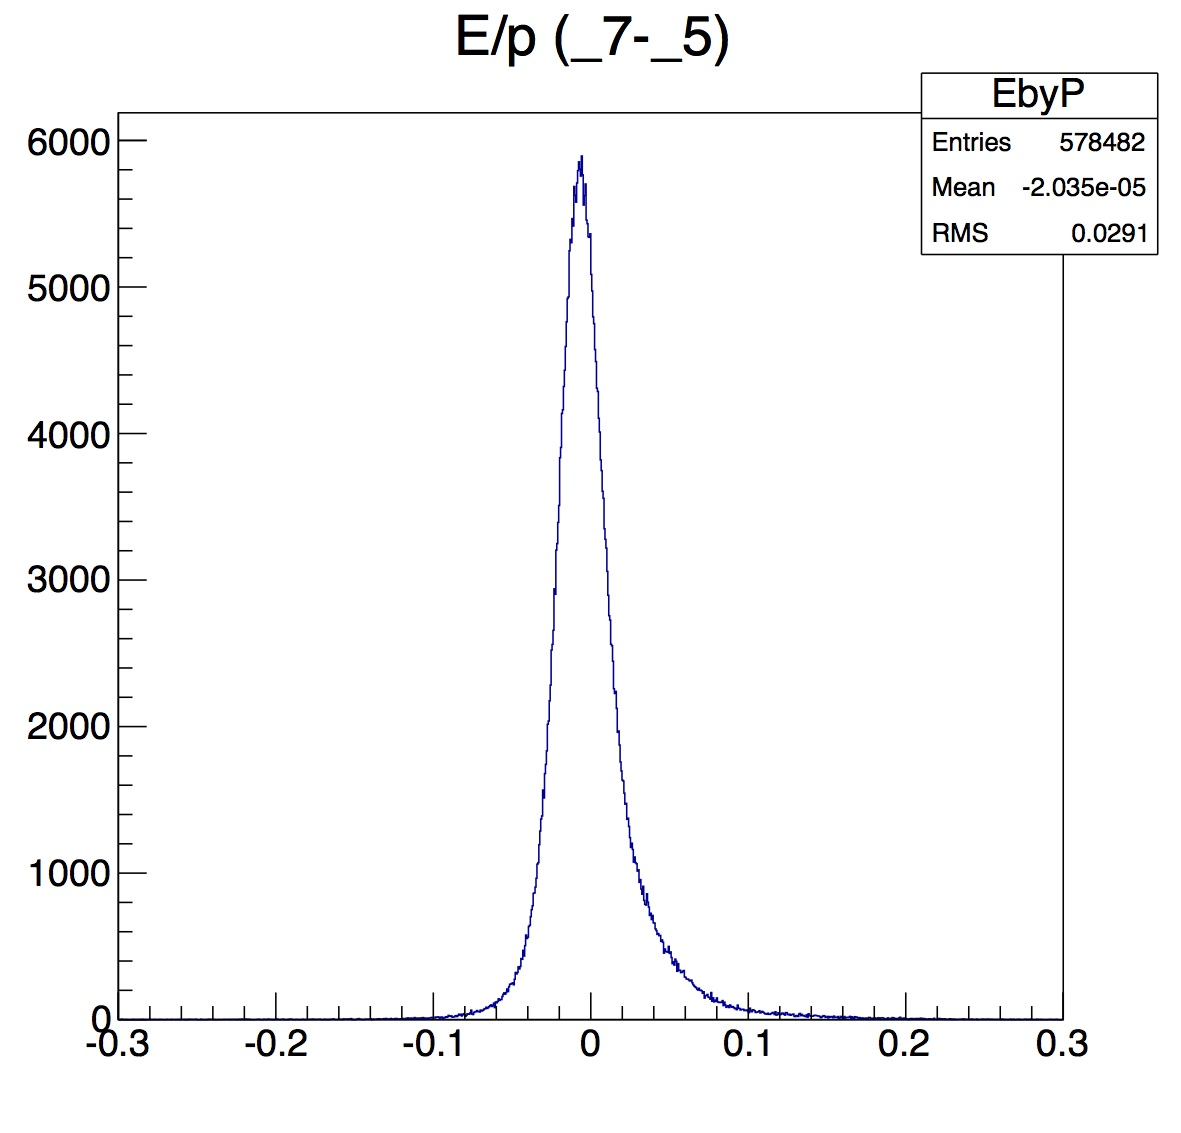
\includegraphics[width=\textwidth]{Plots/EbyP}
                \caption{A tiger}
                \label{fig:tiger}
        \end{subfigure}
  
        \caption{Pictures of animals}\label{fig:animals}
\end{figure}

The quanittiy $E/p$ is important to check because it is used as a direct input into one of the calibration modules. Fig. 9.a) shows the distributions of $E/p$ for all eclectrons in teh sample for each framework: the red histogram represents the distrbution in the 53X framework, while the blue histrogram represents the distribution in the 70X framweok. Only electrons which were matched in both samples were used for these plots. Fig 9.b) represents the differnce between these two quanitities. FIXME why is this importnat?



\subsubsection{$R_9$}
\begin{figure}[h!]
        \centering
        \begin{subfigure}[b]{0.4\textwidth}
                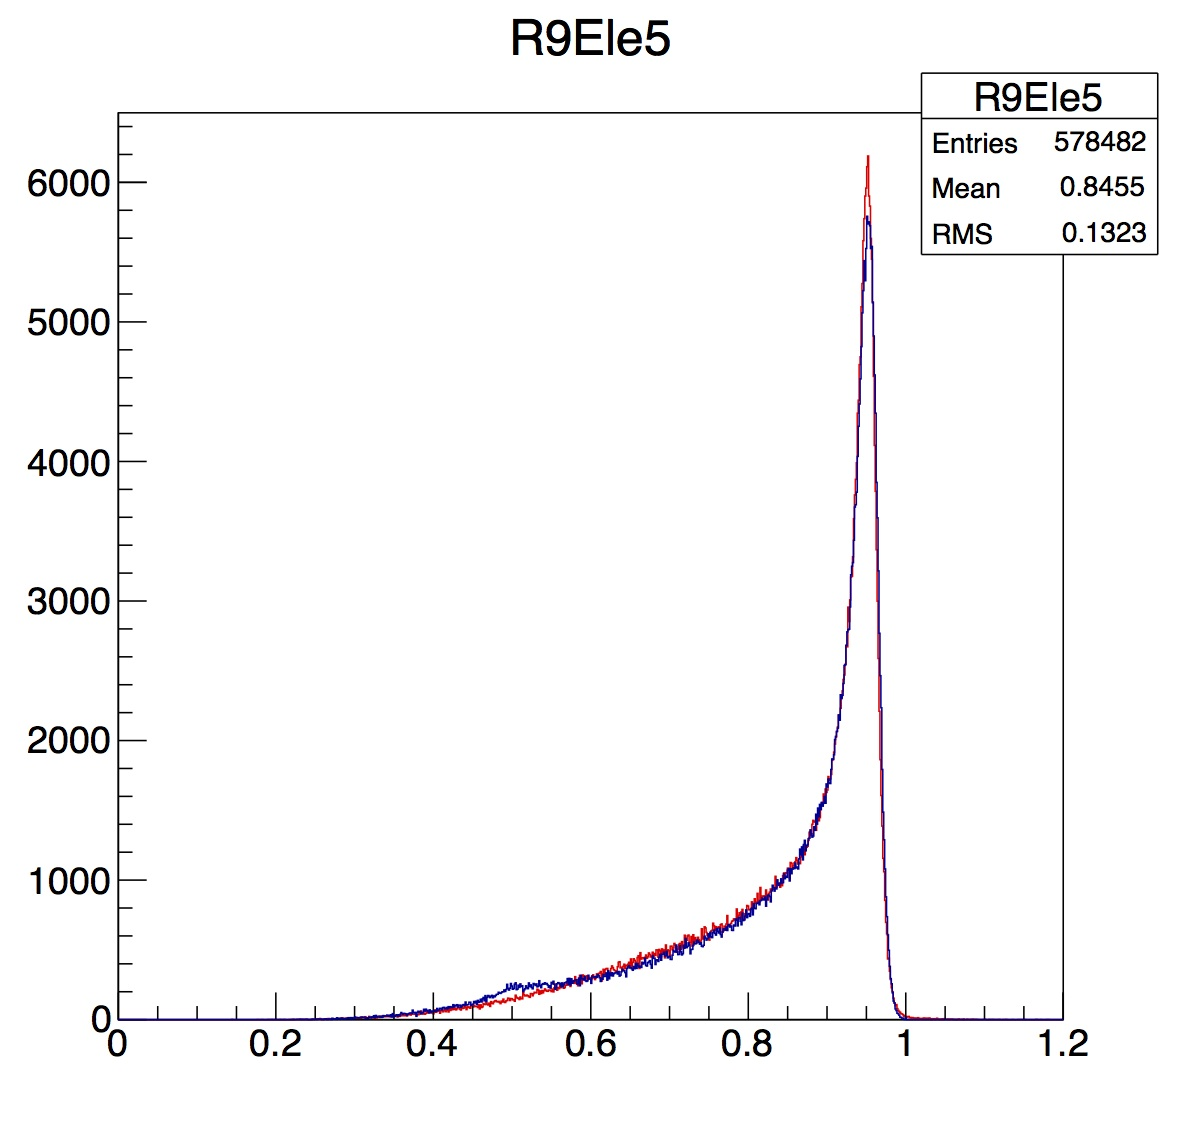
\includegraphics[width=\textwidth]{Plots/R9dist}
                \caption{A gull}
                \label{fig:gull}
        \end{subfigure}%
        ~ %add desired spacing between images, e. g. ~, \quad, \qquad, \hfill etc.
          %(or a blank line to force the subfigure onto a new line)
        \begin{subfigure}[b]{0.4\textwidth}
                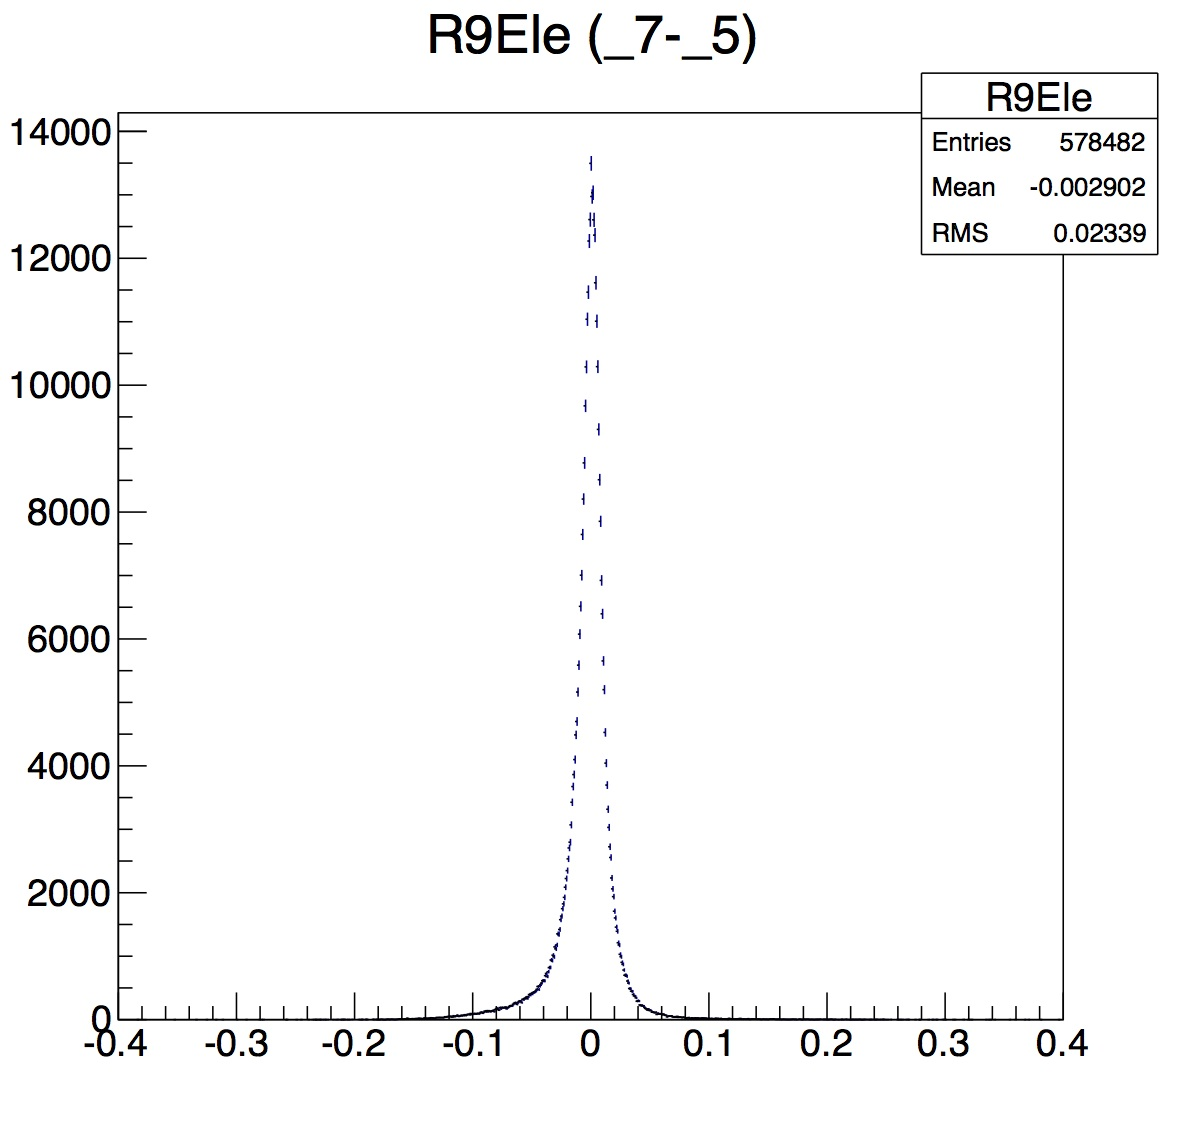
\includegraphics[width=\textwidth]{Plots/R9}
                \caption{A tiger}
                \label{fig:tiger}
        \end{subfigure}
       
        \caption{Pictures of animals}\label{fig:animals}
\end{figure}

For electrons, the interpretation of $R_9$ is different to that for photons. In this case, it indicates whether an electron is likely to have emitted a large fraction of its energy through bremmshtalung or not. electrons with $R_9>0.94$ are likely to have showered little, and are known as ``gold'' electrons. On the other hadn, electrons with $R_9\leq 0.94$ are known as ``bad'' electrons, as they will have little more of theyr energy before hitting the detector. In this cas, they are more difficult to reconstruct. Fig. 9.a) shows the distribution of the $R_9$ of electrons in the data samples. The red line refers to electrons reconstrcuted in 53X, while the blue line shows the distributions of electrons reconstructed in 70X. Only electrons which had a match from one sample to the other were included. The distributions match up well, apart from the peak, where the 70X distribution is not as high, and around 0.5, where the 70X distribution shows a bump. These features needs to be investigated, in order to determine what teh cause is. Fig. 9.b) shows the distibution of the difference in $R_9$ (ie $(R_9)_{70X} -(R_9)_{53X}$). This forms a tight peak around 0, indicative that the two versions are generally assigning the same value of $R_9$ to the electrons.

\subsubsection{Bremmstrahlung fraction}
\begin{figure}[h!]
        \centering
        \begin{subfigure}[b]{0.4\textwidth}
                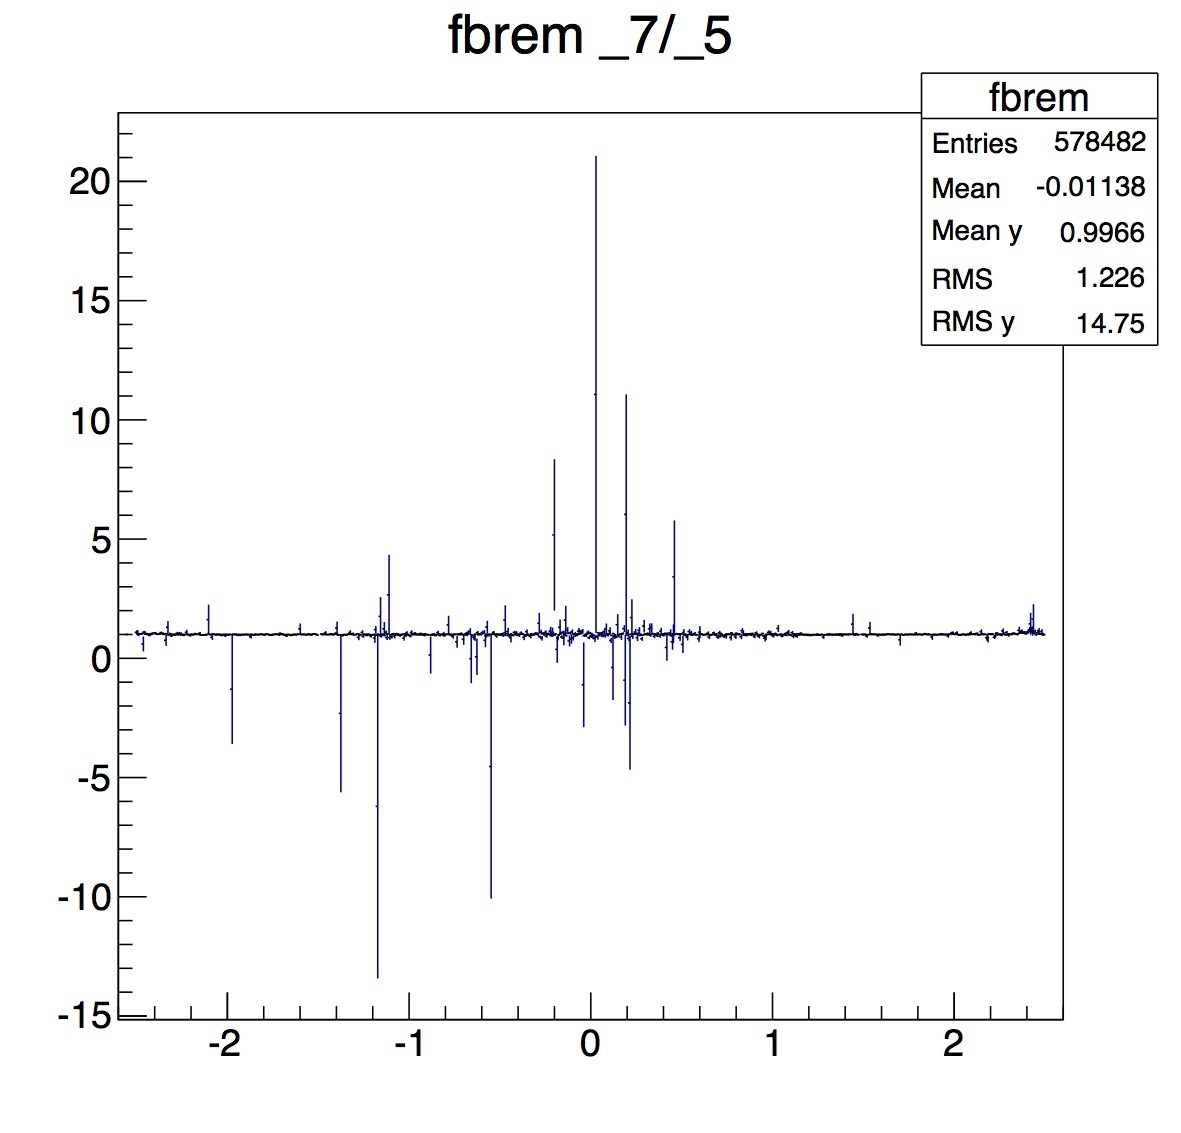
\includegraphics[width=\textwidth]{Plots/fbrem}
                \caption{A gull}
                \label{fig:gull}
        \end{subfigure}%

        \caption{Pictures of animals}\label{fig:animals}
\end{figure}
A related object is the bremmstrahlung fraction $f_{\text{brem}}$, defined $(p_{\text{in}} -p_{\text{out}})/p_{\text{in}}$ (where $p$ is the elctron 4-momentum and the subscirpts ``in'' and ``out'' refer to whetehr the moentum is measured as the electron leaves or enters the tracker (FIXME check!!)). In theory, this quantity should not chnage between 70X and 53X, and indeed Fig. 10 shows that the ratio of the $f_{\text{brem}}$ in 53X and 70X is consistent with 1 across all of $\eta$.

\subsubsection{$\eta,\phi$ coordinates}
\begin{figure}[h!]
        \centering
        \begin{subfigure}[b]{0.22\textwidth}
                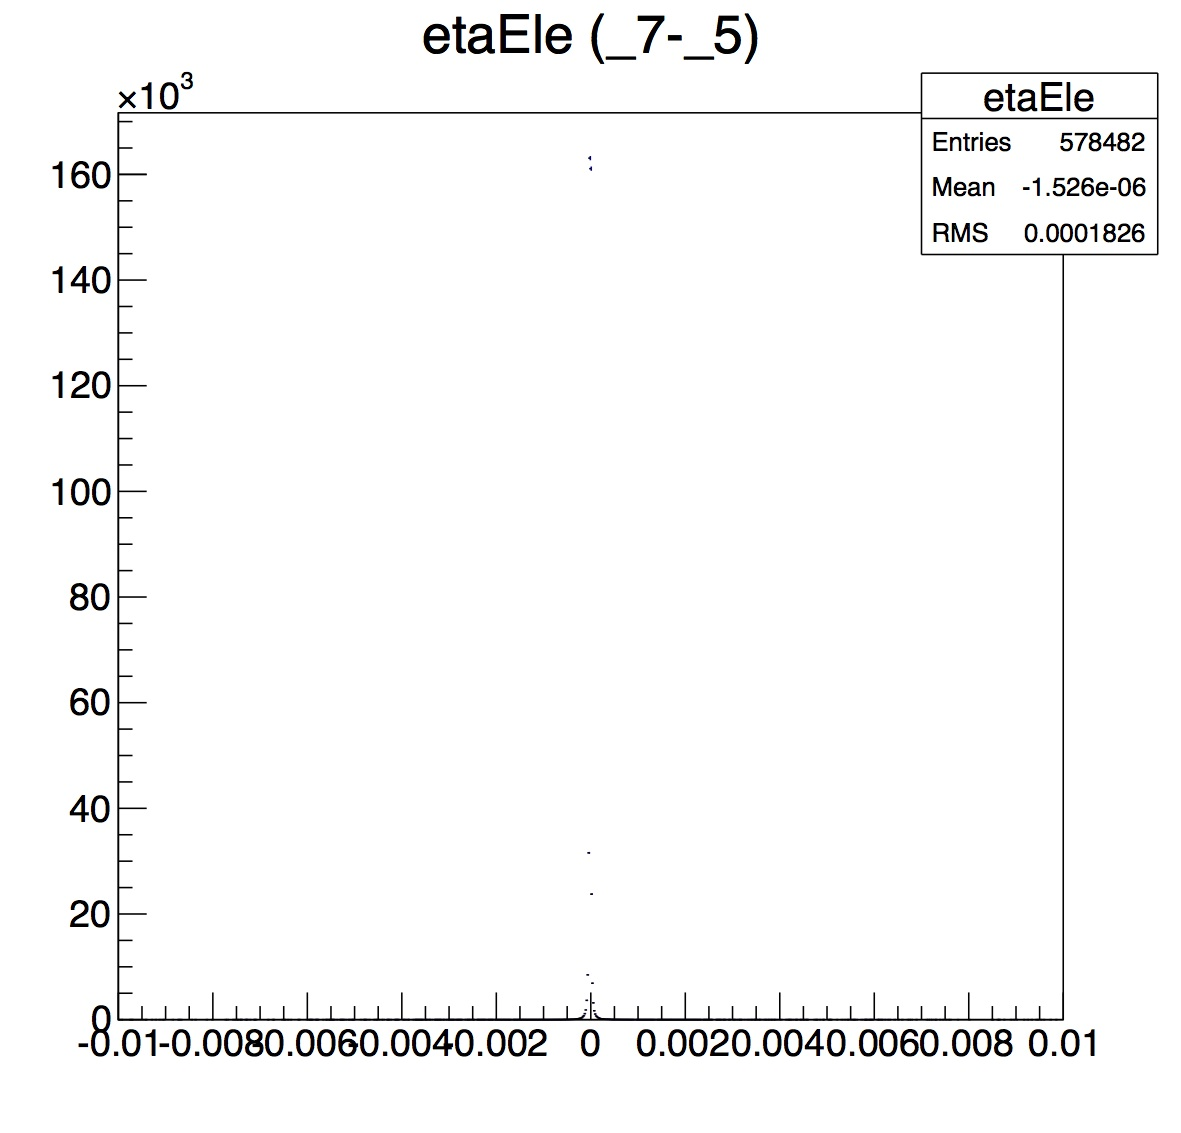
\includegraphics[width=\textwidth]{Plots/eta}
                \caption{A gull}
                \label{fig:gull}
        \end{subfigure}%
        ~ %add desired spacing between images, e. g. ~, \quad, \qquad, \hfill etc.
          %(or a blank line to force the subfigure onto a new line)
        \begin{subfigure}[b]{0.22\textwidth}
                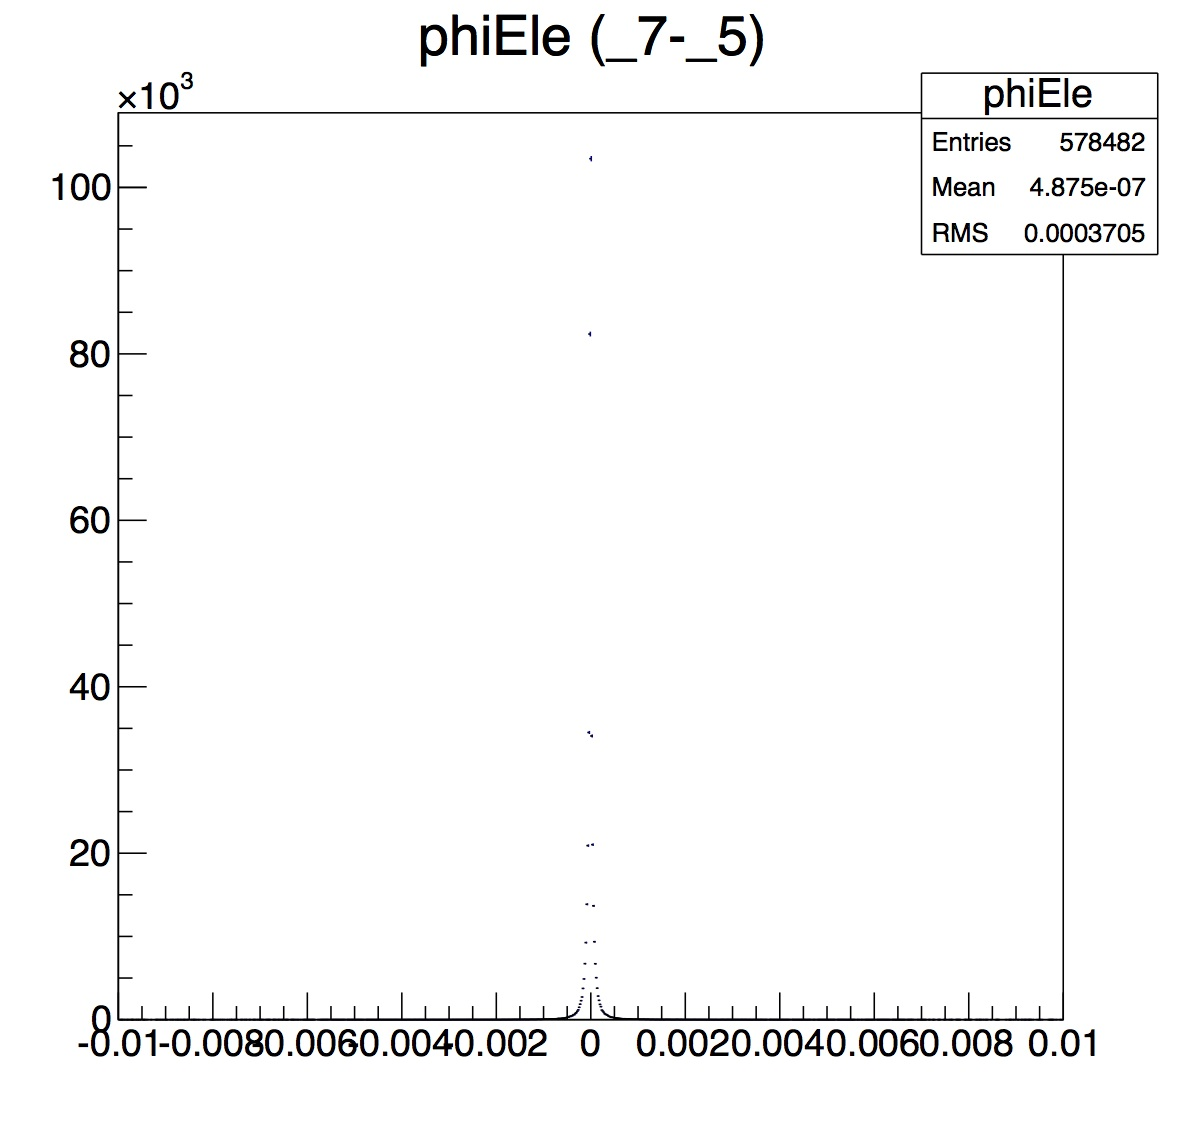
\includegraphics[width=\textwidth]{Plots/phi}
                \caption{A tiger}
                \label{fig:tiger}
        \end{subfigure}
        ~ %add desired spacing between images, e. g. ~, \quad, \qquad, \hfill etc.
          %(or a blank line to force the subfigure onto a new line)
        \begin{subfigure}[b]{0.22\textwidth}
                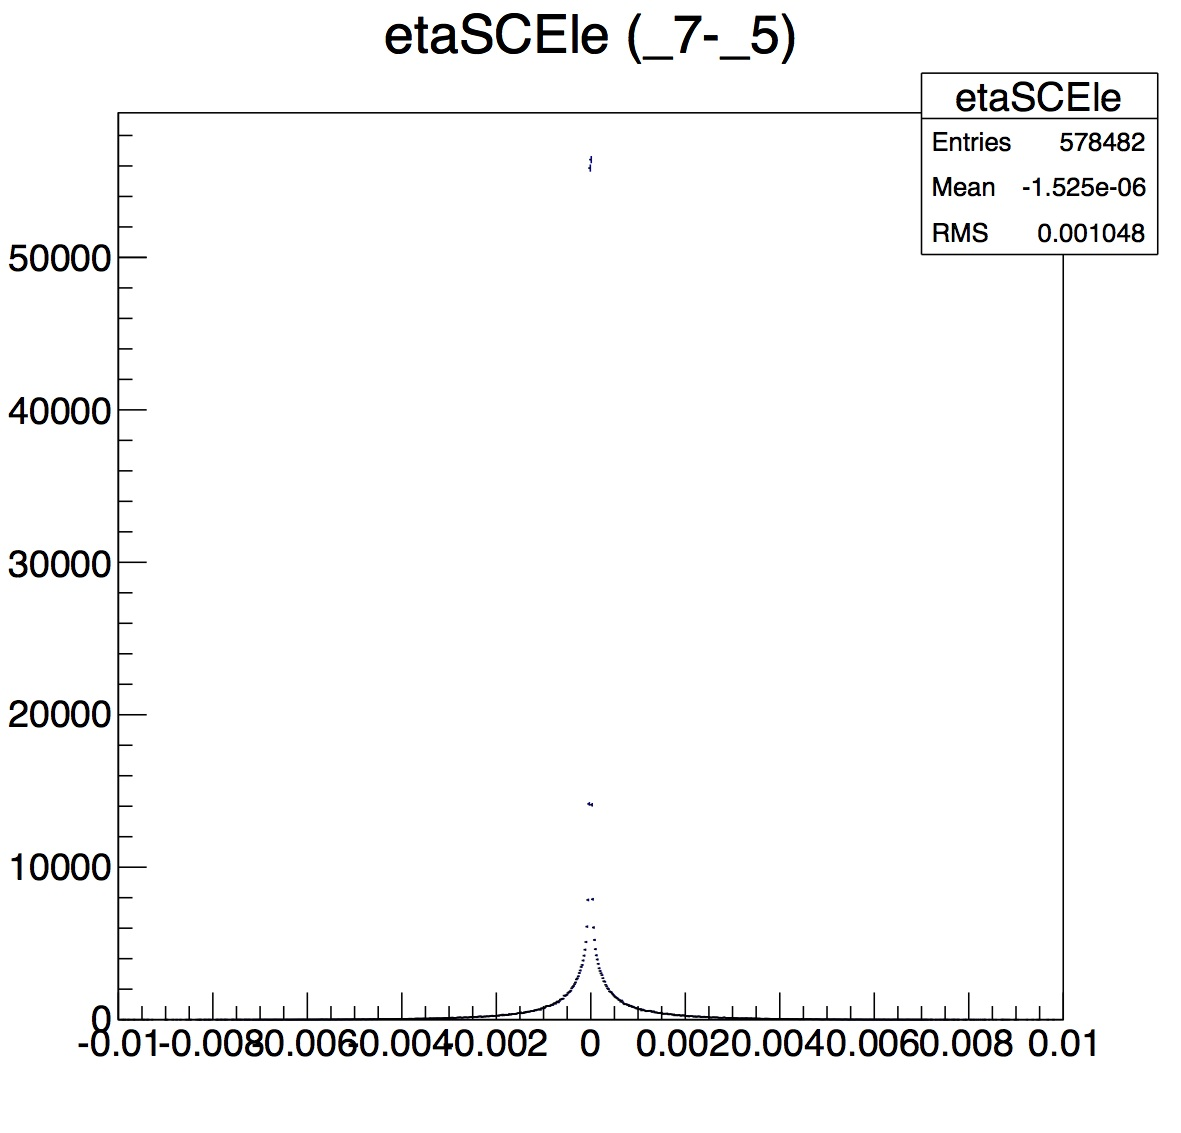
\includegraphics[width=\textwidth]{Plots/etaSC}
                \caption{A mouse}
                \label{fig:mouse}
        \end{subfigure}
         \begin{subfigure}[b]{0.22\textwidth}
                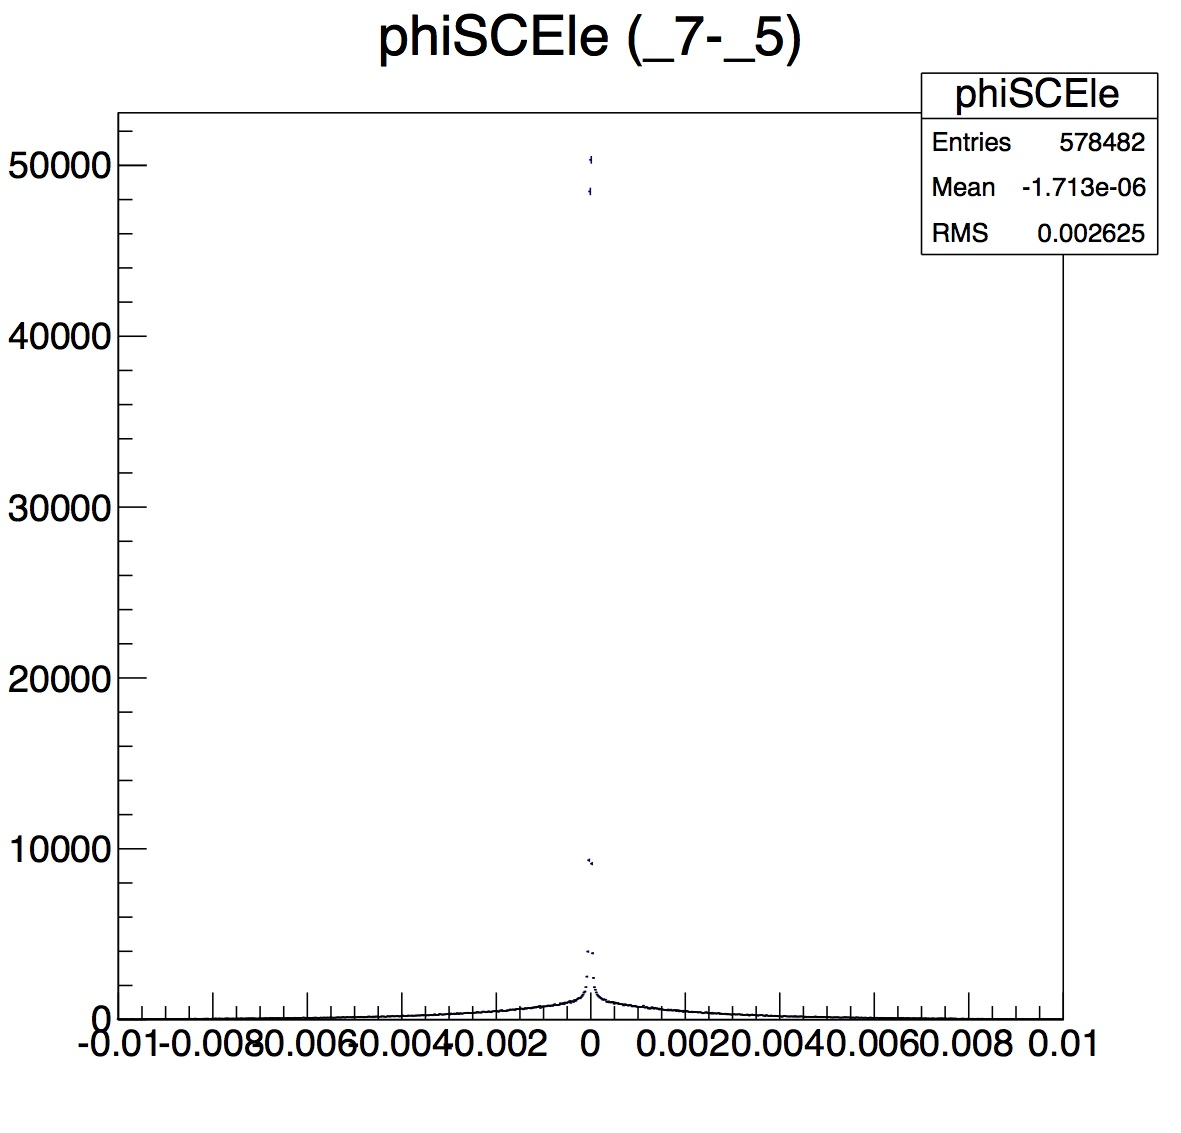
\includegraphics[width=\textwidth]{Plots/phiSC}
                \caption{A mouse}
                \label{fig:mouse}
        \end{subfigure}
        \caption{Pictures of animals}\label{fig:animals}
\end{figure}

The position where the electrons hit the ECAL (known as the supercluster position $\eta_{\text{SC}},\phi_{\text{SC}}$) fshould not be largely affected by the change in framewok, and neither should the coordinates of teh electron tracks (in this case, knwon as $\eta,\phi$  ( the difference between the two is that $\eta_{\text{SC}},\phi_{\text{SC}}$ are measured from the center of the detetcor, while $\eta,\phi$ start at the interaction vertex, and thus are shifted in the $z$-direction). Fig. 12 shows the distributions of the chnage in the value of individual electros' reconstructed $\eta_{\text{SC}},\phi_{\text{SC}},\eta \text{ and } \phi$ respectively. As expected, the distribtuions form extremely narrow peaks around zero. This idcates that indeed, the values of the coordinates remain largely unaffected. The values of $\eta_{\text{SC}},\phi_{\text{SC}}$ are more affected than  $\eta,\phi$ , but this makes sense, since $\eta_{\text{SC}},\phi_{\text{SC}}$  are teh coordinates of the most energetic crystal in the cluster, and thus would be more affected by a chnage in clustering algorithm.


\subsubsection{$Z\rightarrow e^+ e^-$ invariant mass }
\begin{figure}[h!]
        \centering
        \begin{subfigure}[b]{0.8\textwidth}
                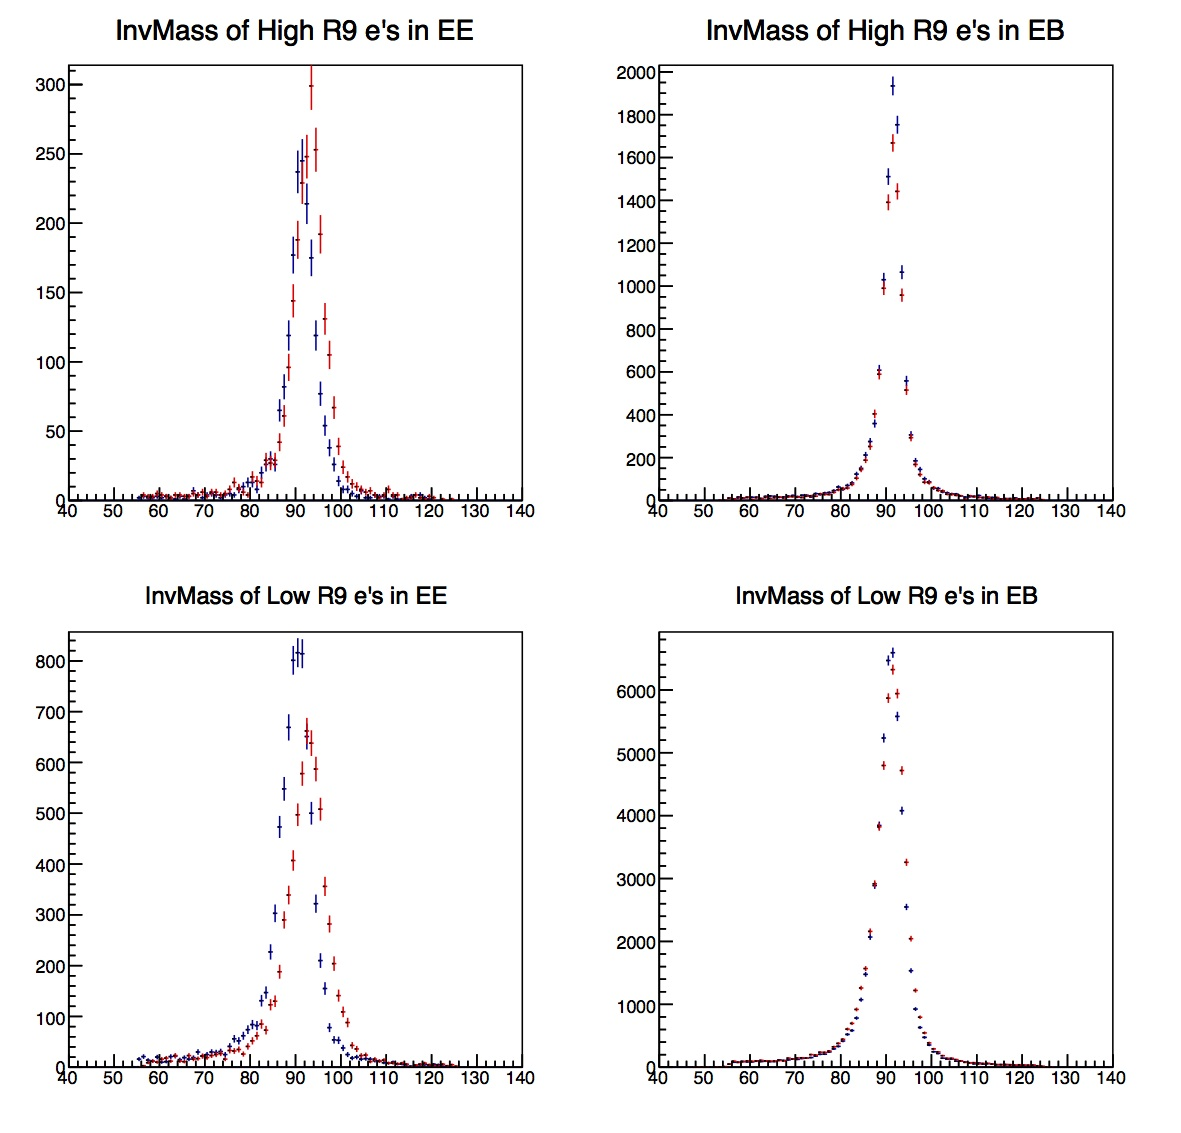
\includegraphics[width=\textwidth]{Plots/Zee_corr}
                \caption{A gull}
                \label{fig:gull}
        \end{subfigure}%
      
        \caption{Pictures of animals}\label{fig:animals}
\end{figure}

Finally, the invariant mass distributions of various categories of $Z \rightarrow e^+e^-$ system are shown. There are four categoreis considered here: a) both resulting electrons have $R_9 >0.94$ and are both in the EE, b) both with $R_9>0.94$ and in the EB, c) both with $R_9 \leq 0.94$ and in EE and d) c) both with $R_9 \leq 0.94$ and in EB. The red lines indicate the distribtuons obtained when considering electrons in the 53X framewroks, while the blue lines represent electrons from the 70X version. Only matched electrons are included in this plot. The Invariant mass is caluclated using the corrected energy of the electrons - the best available for both 70X and 53X. The plots show good agreement in the two EB catgeories, where the two peaks overalp well, apart from the height of the peak. There is however a visible discrepancy in the EE, the the peaks appear shifted with respect to one another. Futrther investogation is needed to undertsand the differences observed.

\subsection{Next Steps}

This section has shown results from the preliminary steps of validation of the regression in the 70X fraework. At the moment, the comaprisons are being made using data reconstructed in both 53X and 70X, but for full validation, matchign MC sampels are needed also. Although some variables appear to match (namely the $\eta_{\text{SC}},\phi_{\text{SC}},\eta \text{ and }\phi$), more studies are needed to probe differences obsevred between energy-based variables. The MC for the 70X sample is due to become available shortly, so we will eb able to run the ECALELF tool in its entirety, and thus provide a better correction for the 70X energy. This new correction should allow a more fair comaprison to be made between 53X and 70X. I am working with the ECAL detector performance group to pursue this work.




\section{Future work}

The $H \rightarrow \gamma \gamma$ working group are in the process of finalising the legacy analysis for the $\sqrt{s}=7$ and $8$ TeV data samples from run I. This will include a mass measurement for the Higgs boson based on a similar analysis to the one described above. An analysis of the spin properties of this particle, which I was involved in, will also be included. This publication will reflect the final word on the older data samples from the perspective of the CMS $H \rightarrow \gamma \gamma$ analysis. The LHC should begin colliding again in 2015, and new data will then become available. Various new measurements will need to be made to further understand the properties of the Higgs boson. Further data will be able to shed light on the existence of a potential second Higgs boson (multiple such bosons are predicted in various BSM frameworks), and will allow precision measurements of differential cross sections, couplings and spin/parity. Deviations from the expected properties of the SM Higgs boson could signal the potential existence of BSM physics.  $H\rightarrow \gamma \gamma$ will remain one of the most sensitive channels with which to analyse the properties of the Higgs during run II.
On a more personal note, my work within the CMS experiement will intially be centred around the ECAL, preparing for calibration in run II. The way that photons are reconstructed is being modified, and I will help determine what the effect of this change will be on the sensitivity of the $H \rightarrow \gamma \gamma$ analysis. As 2015 approaches, I will become involved in planning and implementing the next round of analysis, to help further pin down the properties of the Higgs boson.

\section{Conclusion}

To conclude, it is clear that even though we have now discovered the elusive Higgs boson, many questions remain unanswered. In 2015, some BSM theories which might help to answer these questions will be tested. If nothing is found in direct searches, the precision analysis of the properties of the Higgs boson will be one of key avenues with which to search for deviations from the SM. As such, further understanding of the Higgs boson's properties are not only desirable, but indeed imperative if we are to understand more about the fundamental  structure of the universe.


\bibliographystyle{unsrt}
\bibliography{mybib}
%\end{multicols}
\end{document}